\documentclass[conference]{IEEEtran}
\IEEEoverridecommandlockouts

\usepackage{amsmath}
\usepackage{graphicx}
\usepackage{cite}
% Also needed by the sections: amssymb (\mathbb in Theory), array and booktabs (tables),
% xcolor with table option (row shading), url (bibliography links), tcolorbox (boxes below).
\usepackage{amssymb}
\usepackage{array}
\usepackage{booktabs}
\usepackage[table]{xcolor}
\usepackage{url}
\usepackage{microtype}
\usepackage[most]{tcolorbox}

% Readability: a little more space between lines and paragraphs, fewer stretched lines
\linespread{1.06}
\setlength{\parskip}{3pt plus 1pt}
\setlength{\emergencystretch}{1.5em}
\raggedbottom  % no stretched gaps when a column ends early

% One muted accent for our own-work notes; neutral shading elsewhere
\definecolor{accent}{HTML}{3D5A80}
\definecolor{tblhead}{HTML}{E9ECEF}
\definecolor{tblours}{HTML}{FFF3BF}

% Key results in the Theory section: a light neutral frame
\newcommand{\keyeq}[1]{\tcbhighmath[colback=black!3, colframe=black!30, boxrule=0.4pt, arc=1.5pt,
  left=2pt, right=2pt, top=1pt, bottom=1pt]{#1}}
% "In our project" notes: how the theory applies to our settings
\newtcolorbox{projectbox}{enhanced, breakable, colback=accent!4!white, colframe=accent!70,
  boxrule=0.5pt, arc=1.5pt, left=5pt, right=5pt, top=3pt, bottom=4pt, before skip=8pt, after skip=8pt,
  title={In our project}, fonttitle=\small\bfseries, coltitle=white, colbacktitle=accent!85,
  toptitle=1pt, bottomtitle=1pt}
\newcommand{\relevance}{\textit{Relevance:}}

% Clickable references, citations and links, plus a section outline in the PDF viewer (load last)
\usepackage[colorlinks=true, linkcolor=accent, citecolor=accent, urlcolor=accent,
  bookmarks=true, bookmarksnumbered=true, pdftitle={Next Day Wildfire Spread Prediction}]{hyperref}

% Overleaf: figures/ sits next to main.tex. In the repo, figures resolve from ../reports/figures/.
\graphicspath{{./}{../reports/}}

\begin{document}

\title{Next Day Wildfire Spread Prediction}

\author{
\IEEEauthorblockN{Harshil, Sushant, Priyanshu, Sachin, Piyush}
\IEEEauthorblockA{CS \& AI Department, Rishihood University}
}

\maketitle
\thispagestyle{plain}
\pagestyle{plain}

% Abstract as a heading with plain text below (instead of IEEE's inline bold "Abstract-")
\section*{Abstract}
We predict which areas an active wildfire will burn the next day, using the Next Day Wildfire Spread
dataset (18\,545 U.S.\ fire events at 1\,km resolution), where only 1.1\% of pixels burn on day $t+1$. We
keep a per-pixel model and add 23 engineered spatial features, such as distance to the nearest fire and
fire upwind. Tuned XGBoost reaches a test PR AUC of 0.257, compared with 0.106 for persistence. The
dataset authors report 0.225 for a random forest and 0.284 for a CNN, from a different training pipeline,
so these are reference points rather than a controlled comparison. Ablation shows that the spatial features
carry the signal, while tuning changes the score by only about 0.01. The model finds fire near the
existing front but misses spread beyond 5\,km, which motivates a spatial deep model in Phase~2.

\noindent\textit{Index terms:} wildfire spread, remote sensing, gradient boosting, class imbalance,
precision-recall.

% Introduction
% Numbers come from reports/results_table.md, reports/ablation.csv and the other sections.

\section{Introduction}
\label{sec:intro}

Once a wildfire is burning, the question that matters for the next day is where it will spread.
Knowing which areas are likely to burn helps crews and resources be placed ahead of the fire front.
Physics-based simulators answer this from fuel, weather and terrain~\cite{rothermel1972}, but they need
detailed fuel descriptions and are not fitted to observed fires. Satellites now record active fires
daily, so the question can also be posed as a learning problem: given today's fire and conditions,
predict tomorrow's fire.

We study this problem on the Next Day Wildfire Spread (NDWS) dataset of Huot
et al.~\cite{huot2022}. It contains 18\,545 samples over the contiguous United States from 2012 to
2020, each a $64\times64$\,km patch at 1\,km resolution. The authors call them fire events, but one
fire can appear in several overlapping samples (Section~\ref{sec:events}). Each patch has 12 inputs on day $t$ (the active
fire mask plus weather, drought, vegetation, terrain and population) and the fire mask on day $t+1$ as
the label. Two properties make the task hard. First, it is extremely imbalanced: only 1.1\% of labelled
training pixels burn the next day, so a model that never predicts fire is already more than 98\%
accurate. Second, the signal is spatial: a pixel's own weather says little about whether it will
burn, while nearby fire and wind direction say a great deal. In the dataset paper, a convolutional
network that sees the whole patch clearly beats pixel models that see only a pixel and its eight
neighbours, and later U-Net and transformer models report higher scores still
(Section~\ref{sec:related}).

Phase~1 of our project asks how far classical machine learning can go when it is given the right
spatial information. We keep a per-pixel model, which is fast to train and easy to inspect, and move
the spatial reasoning into engineered features. Gradient-boosted trees then learn from these features.
Fig.~\ref{fig:pipeline} shows the pipeline. Our contributions are:

\begin{figure*}[t]
\centering
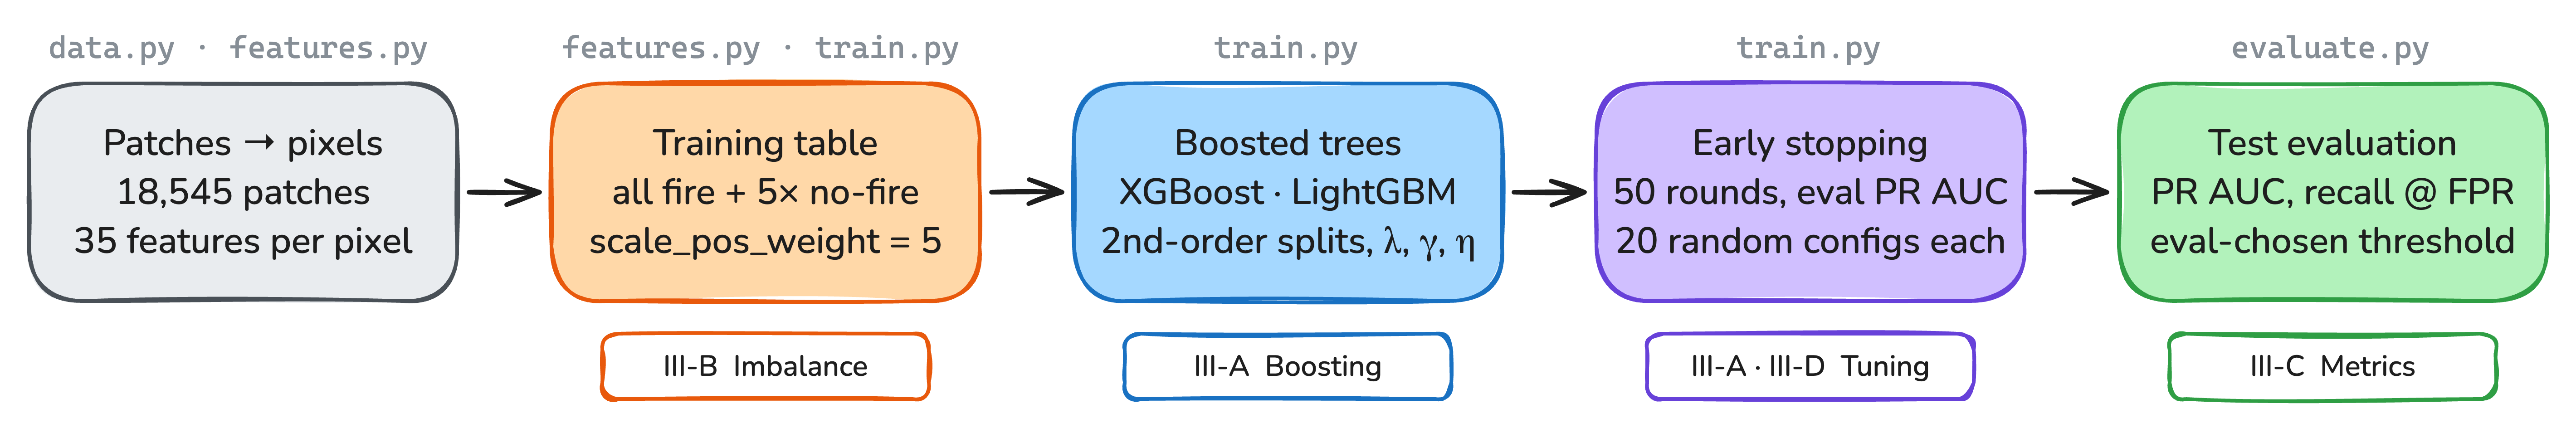
\includegraphics[width=\textwidth]{figures/th_pipeline.png}
\caption{Our Phase~1 pipeline (\texttt{src/}). Each tag names the part of Section~\ref{sec:theory} that
explains that step.}
\label{fig:pipeline}
\end{figure*}
\begin{itemize}
\item a TensorFlow-free data pipeline with physical clipping of export artefacts, and the finding that
the patches are stored south-up, which every direction-dependent feature relies on;
\item 23 engineered features in five groups, including fire density at three scales, distance to the
nearest fire, fire upwind at up to 8\,km, and vapour pressure deficit;
\item tuned XGBoost and LightGBM models whose test PR AUC (0.257 and 0.248) lies between the dataset
authors' pixel models and their CNN;
\item an analysis of what the model learns and where it fails: a feature-group ablation, SHAP values,
a downwind plausibility check, error analysis and an evaluation by fire event.
\end{itemize}

Section~\ref{sec:related} reviews related work, and Section~\ref{sec:theory} gives the theory behind
our modelling choices. The following sections describe the dataset and exploratory analysis, the
methodology and feature engineering, and the results. The last section concludes and outlines
Phase~2.

% Related Work (Priyanshu)
% Uses \relevance and projectbox from main.tex. Every paper fact was checked against the paper itself,
% its DOI / proceedings page or its official data record. Our numbers come from reports/results_table.md.
% Figure: figures/rw_context_ladder.png.

\section{Related Work}
\label{sec:related}

We review the literature in four steps: the physics-based model that learned models aim to replace,
machine learning in wildfire science, learned spread models on NDWS and related datasets, and the methods
our pipeline is built on. Table~\ref{tab:relwork} compares the spread studies, and
Section~\ref{sec:rw_position} places our work among them.

\subsection{Physics-based fire spread}

\textbf{Rothermel~\cite{rothermel1972}} developed the surface fire spread model that still underlies U.S.\
fire behaviour tools. Andrews~\cite{andrews2018} describes it as quasi-empirical. It combines a heat-balance
formulation with wind-tunnel experiments in artificial fuel beds and grassfire observations. The model
computes the steady-state rate of spread of a fire front through a uniform fuel bed. Its inputs are fuel
load, depth, surface-area-to-volume ratio, heat content, mineral content, moisture and moisture of
extinction, together with midflame wind speed and slope. It was first used in the 1972 U.S.\ National
Fire Danger Rating System (NFDRS) and is built into BehavePlus and FARSITE~\cite{andrews2018}.
\relevance{} the energy release component (\texttt{erc}) in our data is an NFDRS output. Our features
use the same drivers (wind, slope, dryness), but leave the form of the relationship to the learner.

\subsection{Machine learning in wildfire science}

\textbf{Jain et al.~\cite{jain2020}} review machine learning in wildfire science and management. They find
300 publications up to the end of 2019. Fire occurrence, susceptibility and risk is the largest domain
(127 papers), and fire behaviour prediction, which includes spread, has 43. Random forests, MaxEnt,
neural networks, decision trees, SVMs and genetic algorithms are the most common methods.
\relevance{} spread prediction is a small part of the field.

\textbf{Sayad et al.~\cite{sayad2019}} predict wildfire \emph{occurrence} from three MODIS products (NDVI,
land surface temperature, thermal anomalies) over central Canada. Their table has 804 rows (386 fire, 418
no fire), and an ANN and an SVM reach 98.32\% accuracy. \relevance{} with balanced classes, accuracy is
informative. On our test split, 98.75\% of pixels do not burn, so accuracy is not.

\subsection{Learned spread models on other data}

\textbf{Hodges and Lattimer~\cite{hodges2019}} train a deep convolutional inverse graphics network to
reproduce simulated burn maps (Rothermel's equations and FARSITE) every 6\,h up to 24\,h. They report
precision, sensitivity, F-measure and Chan-Vese similarity of 0.97, 0.92, 0.93 and 0.93 against the
simulator, at a computational cost three orders of magnitude lower. \relevance{} these scores measure
agreement with a simulator, not with observed fires.

\textbf{Radke et al.~\cite{radke2019}} (FireCast) predict 24\,h spread from GeoMAC perimeters of Rocky
Mountain fires since 2013, Landsat-8 imagery, elevation and weather, using a CNN on a window around each
pixel. On the 2016 Beaver Creek fire they report 87.7\% accuracy and 91.1\% recall, but 3.6\% precision
and a 6.4\% F-score. \relevance{} when fire is rare, accuracy and recall can hide very low precision.

\textbf{Gerard et al.~\cite{gerard2023}} build WildfireSpreadTS, a multi-day dataset of 13\,607 VIIRS
images (375\,m) of 607 U.S.\ fires from 2018 to 2021, scored by average precision over 12 year-based folds.
Persistence reaches 0.193, logistic regression up to 0.288, a ResNet-18 U-Net 0.341, and a temporal
attention U-Net (UTAE) with five input days 0.372. \relevance{} a different sensor and split, but the same
ordering: spatial and temporal models beat pixel models.

\subsection{Learned spread models on NDWS}

\textbf{Huot et al.~\cite{huot2022}} introduce Next Day Wildfire Spread (NDWS): 18\,545 fire events over
the contiguous U.S.\ (2012-2020), each a $64\times64$\,km patch at 1\,km with 12 day-$t$ inputs and the
day-$(t{+}1)$ MODIS fire mask. Whole weeks are assigned to train, eval and test in an 8:1:1 ratio. On PR
AUC, persistence scores 0.115, logistic regression 0.198, and a random forest of depth 15 scores 0.225;
both pixel models see each pixel and its eight neighbours. A convolutional autoencoder that sees the
whole patch reaches 0.284. \relevance{} we use their data, split and metric.

\textbf{Fitzgerald et al.~\cite{fitzgerald2023}} add attention blocks to a U-Net and train it with focal
loss on random $32\times32$ crops, discarding crops with uncertain labels. The best model reaches F1
0.370; no PR AUC is reported. They also note that most next-day fire lies in the patch centre and that
models learn to predict fire there. \relevance{} cropped, filtered test sets give numbers that cannot be
compared with full-patch results.

\textbf{Xiao et al.~\cite{xiao2024}} propose an attention U$^2$-Net and report F1 0.405. They re-split
all 18\,545 samples at random 8:1:1 instead of using the official week-based split, and fill uncertain
labels with 0. \relevance{} a random re-split can place samples of the same fire in training and test.

\textbf{Andrianarivony and Akhloufi~\cite{andrianarivony2025}} (LinU-Mamba) use the official split and
report F1 $42.22 \pm 0.29$ over 10 runs, with uncertain labels clamped to 0 and no PR AUC. Retraining
earlier models on the full split, they find much lower F1 than those papers reported on subsets (20.06
instead of 70.97 for a multi-kernel CNN~\cite{marjani2023}). \relevance{} evaluation protocol changes the
numbers as much as the model does.

\textbf{Zhou et al.~\cite{zhou2025}} compare an autoencoder, ResNet, U-Net and Swin-UNet on $32\times32$
crops; the split is not stated. Swin-UNet reaches PR AUC 0.280 and U-Net 0.274, and an XGBoost baseline,
whose setup is not described, reaches 0.06. \relevance{} the only other tree model on NDWS we found; our
per-pixel XGBoost reaches 0.257 with engineered spatial features.

\textbf{Two recent preprints} report PR AUC on full patches with uncertain labels excluded.
\textbf{Esparza et al.~\cite{esparza2026}} use the official split, choose the threshold on training and
eval data only, and give bootstrap intervals. Their re-run of the convolutional autoencoder reaches 0.327
and a U-Net 0.346, and their best ensemble 0.379. \textbf{Han et al.~\cite{han2026}} (FireSenseNet) report
PR AUC 0.3435, but choose their F1 threshold on the test set. They also show that predicting the union of
both days' fire and setting uncertain labels to 0 inflate F1 by 44-50\%, as in~\cite{luo2026}.
\relevance{} these are the closest comparisons to our protocol, but neither is peer-reviewed.

\begin{table*}[t]
\centering
\caption{Spread studies at a glance. Only rows with the same data, split and metric are comparable; the
protocol column gives the differences. Preprints are marked $^\dagger$.}
\label{tab:relwork}
\small
\setlength{\tabcolsep}{4pt}
\renewcommand{\arraystretch}{1.12}
\newcolumntype{L}[1]{>{\raggedright\arraybackslash}p{#1}}
\begin{tabular}{L{3.4cm}L{3.6cm}L{5.0cm}L{1.9cm}L{2.3cm}}
\toprule
\rowcolor{tblhead}
\textbf{Paper} & \textbf{Method} & \textbf{Data / protocol} & \textbf{Metric} & \textbf{Result} \\
\midrule
Hodges \& Lattimer 2019~\cite{hodges2019} & CNN (DCIGN) & simulated burn maps & F vs.\ simulator & 0.93 \\
Radke et al.\ 2019~\cite{radke2019} & CNN + weather & GeoMAC/Landsat-8, Rocky Mts.\ & Precision / recall & 3.6\% / 91.1\% \\
Gerard et al.\ 2023~\cite{gerard2023} & U-Net / UTAE & WildfireSpreadTS, VIIRS 375\,m & AP & 0.341 / 0.372 \\
\midrule
Huot et al.\ 2022~\cite{huot2022} & Persistence / LR / RF & NDWS official split; LR, RF use 3$\times$3 window & PR AUC & 0.115 / 0.198 / 0.225 \\
Huot et al.\ 2022~\cite{huot2022} & Conv.\ autoencoder & NDWS official split & PR AUC & 0.284 \\
Zhou et al.\ 2025~\cite{zhou2025} & U-Net / Swin-UNet / XGBoost & NDWS, $32\times32$ crops, split not stated & PR AUC & 0.274 / 0.280 / 0.06 \\
Esparza et al.\ 2026$^\dagger$~\cite{esparza2026} & Conv.\ AE / U-Net & NDWS official split, full patches & PR AUC & 0.327 / 0.346 \\
Han et al.\ 2026$^\dagger$~\cite{han2026} & Dual-branch CNN & NDWS 8:1:1, F1 threshold on test & PR AUC & 0.3435 \\
Fitzgerald et al.\ 2023~\cite{fitzgerald2023} & Attention U-Net & NDWS, $32\times32$ crops, uncertain crops dropped & F1 & 0.370 \\
Xiao et al.\ 2024~\cite{xiao2024} & Attention U$^2$-Net & NDWS random re-split, uncertain $\to$ 0 & F1 & 0.405 \\
Andrianarivony \& Akhloufi 2025~\cite{andrianarivony2025} & LinU-Mamba & NDWS official split, uncertain $\to$ 0 & F1 & 0.422 \\
\rowcolor{tblours}
\textbf{Ours} & \textbf{XGBoost, 35 features} & \textbf{NDWS official split, full patches} & \textbf{PR AUC} & \textbf{0.257} \\
\bottomrule
\end{tabular}
\end{table*}

\subsection{Methods we build on}

\textbf{Gradient-boosted trees.} Friedman~\cite{friedman2001} frames boosting as gradient descent in
function space, with regression trees as base learners. Chen and Guestrin~\cite{chen2016} add a
regularised objective and second-order split finding in XGBoost, our main model. Ke et
al.~\cite{ke2017} speed up histogram-based boosting with gradient-based sampling and feature bundling in
LightGBM, our second model, which trains up to more than 20 times faster at similar accuracy. Breiman's
random forests~\cite{breiman2001} average decorrelated trees; they are the strongest pixel model of Huot et
al. Section~\ref{sec:theory_gb} explains how these ideas set our hyperparameters.

\textbf{Segmentation networks.} Ronneberger et al.~\cite{ronneberger2015} propose U-Net, an
encoder-decoder with skip connections for segmentation with few labelled images; it won the ISBI 2015
cell-tracking challenge on two datasets. It is the base of most NDWS models above and a candidate for our
Phase~2.

\textbf{Learning and evaluating under imbalance.} Focal loss~\cite{lin2017} down-weights easy examples,
the alternative to class weighting discussed in Section~\ref{sec:theory_imb}. Davis and
Goadrich~\cite{davis2006} prove that one curve dominates in ROC space if and only if it dominates in PR
space and that PR curves must not be interpolated linearly, and Saito and Rehmsmeier~\cite{saito2015}
show that ROC plots can mislead on imbalanced data. Both support PR AUC as our metric
(Section~\ref{sec:theory_pr}).

\textbf{Interpretation.} SHAP~\cite{lundberg2017} attributes a prediction to features with Shapley
values, and TreeSHAP~\cite{lundberg2020} computes them exactly for tree ensembles. Our Results section uses
them to check that the model's dependence on fire distance, dryness and wind is physically sensible.

\subsection{Where our work sits}
\label{sec:rw_position}

\begin{projectbox}
Three points stand out from Table~\ref{tab:relwork} and Fig.~\ref{fig:rw_ladder}.

\textbf{Protocols differ.} Crops, the handling of uncertain labels, splits and test-set thresholds change
the reported numbers. Only Huot et al.\ and Esparza et al.\ clearly use the official split with full
patches and PR AUC, the protocol we follow.

\textbf{Spatial features help trees.} The NDWS work we found is almost entirely deep spatial models.
Trees appear only as Huot et al.'s neighbour-window baselines (0.225) and as an XGBoost baseline at 0.06. Our
per-pixel XGBoost with engineered spatial features reaches 0.257, above both, and the ablation traces this
to the fire-neighbourhood features.

\textbf{Spatial models are still ahead.} Huot et al.'s CNN (0.284) and recent U-Nets (0.346 in a
preprint) score higher. This gap is what motivates Phase~2: a spatial model that sees the whole patch and
the shape of the fire front. As in the papers above, we have not checked whether one fire can appear in
more than one split.
\end{projectbox}

\begin{figure}[t]
\centering
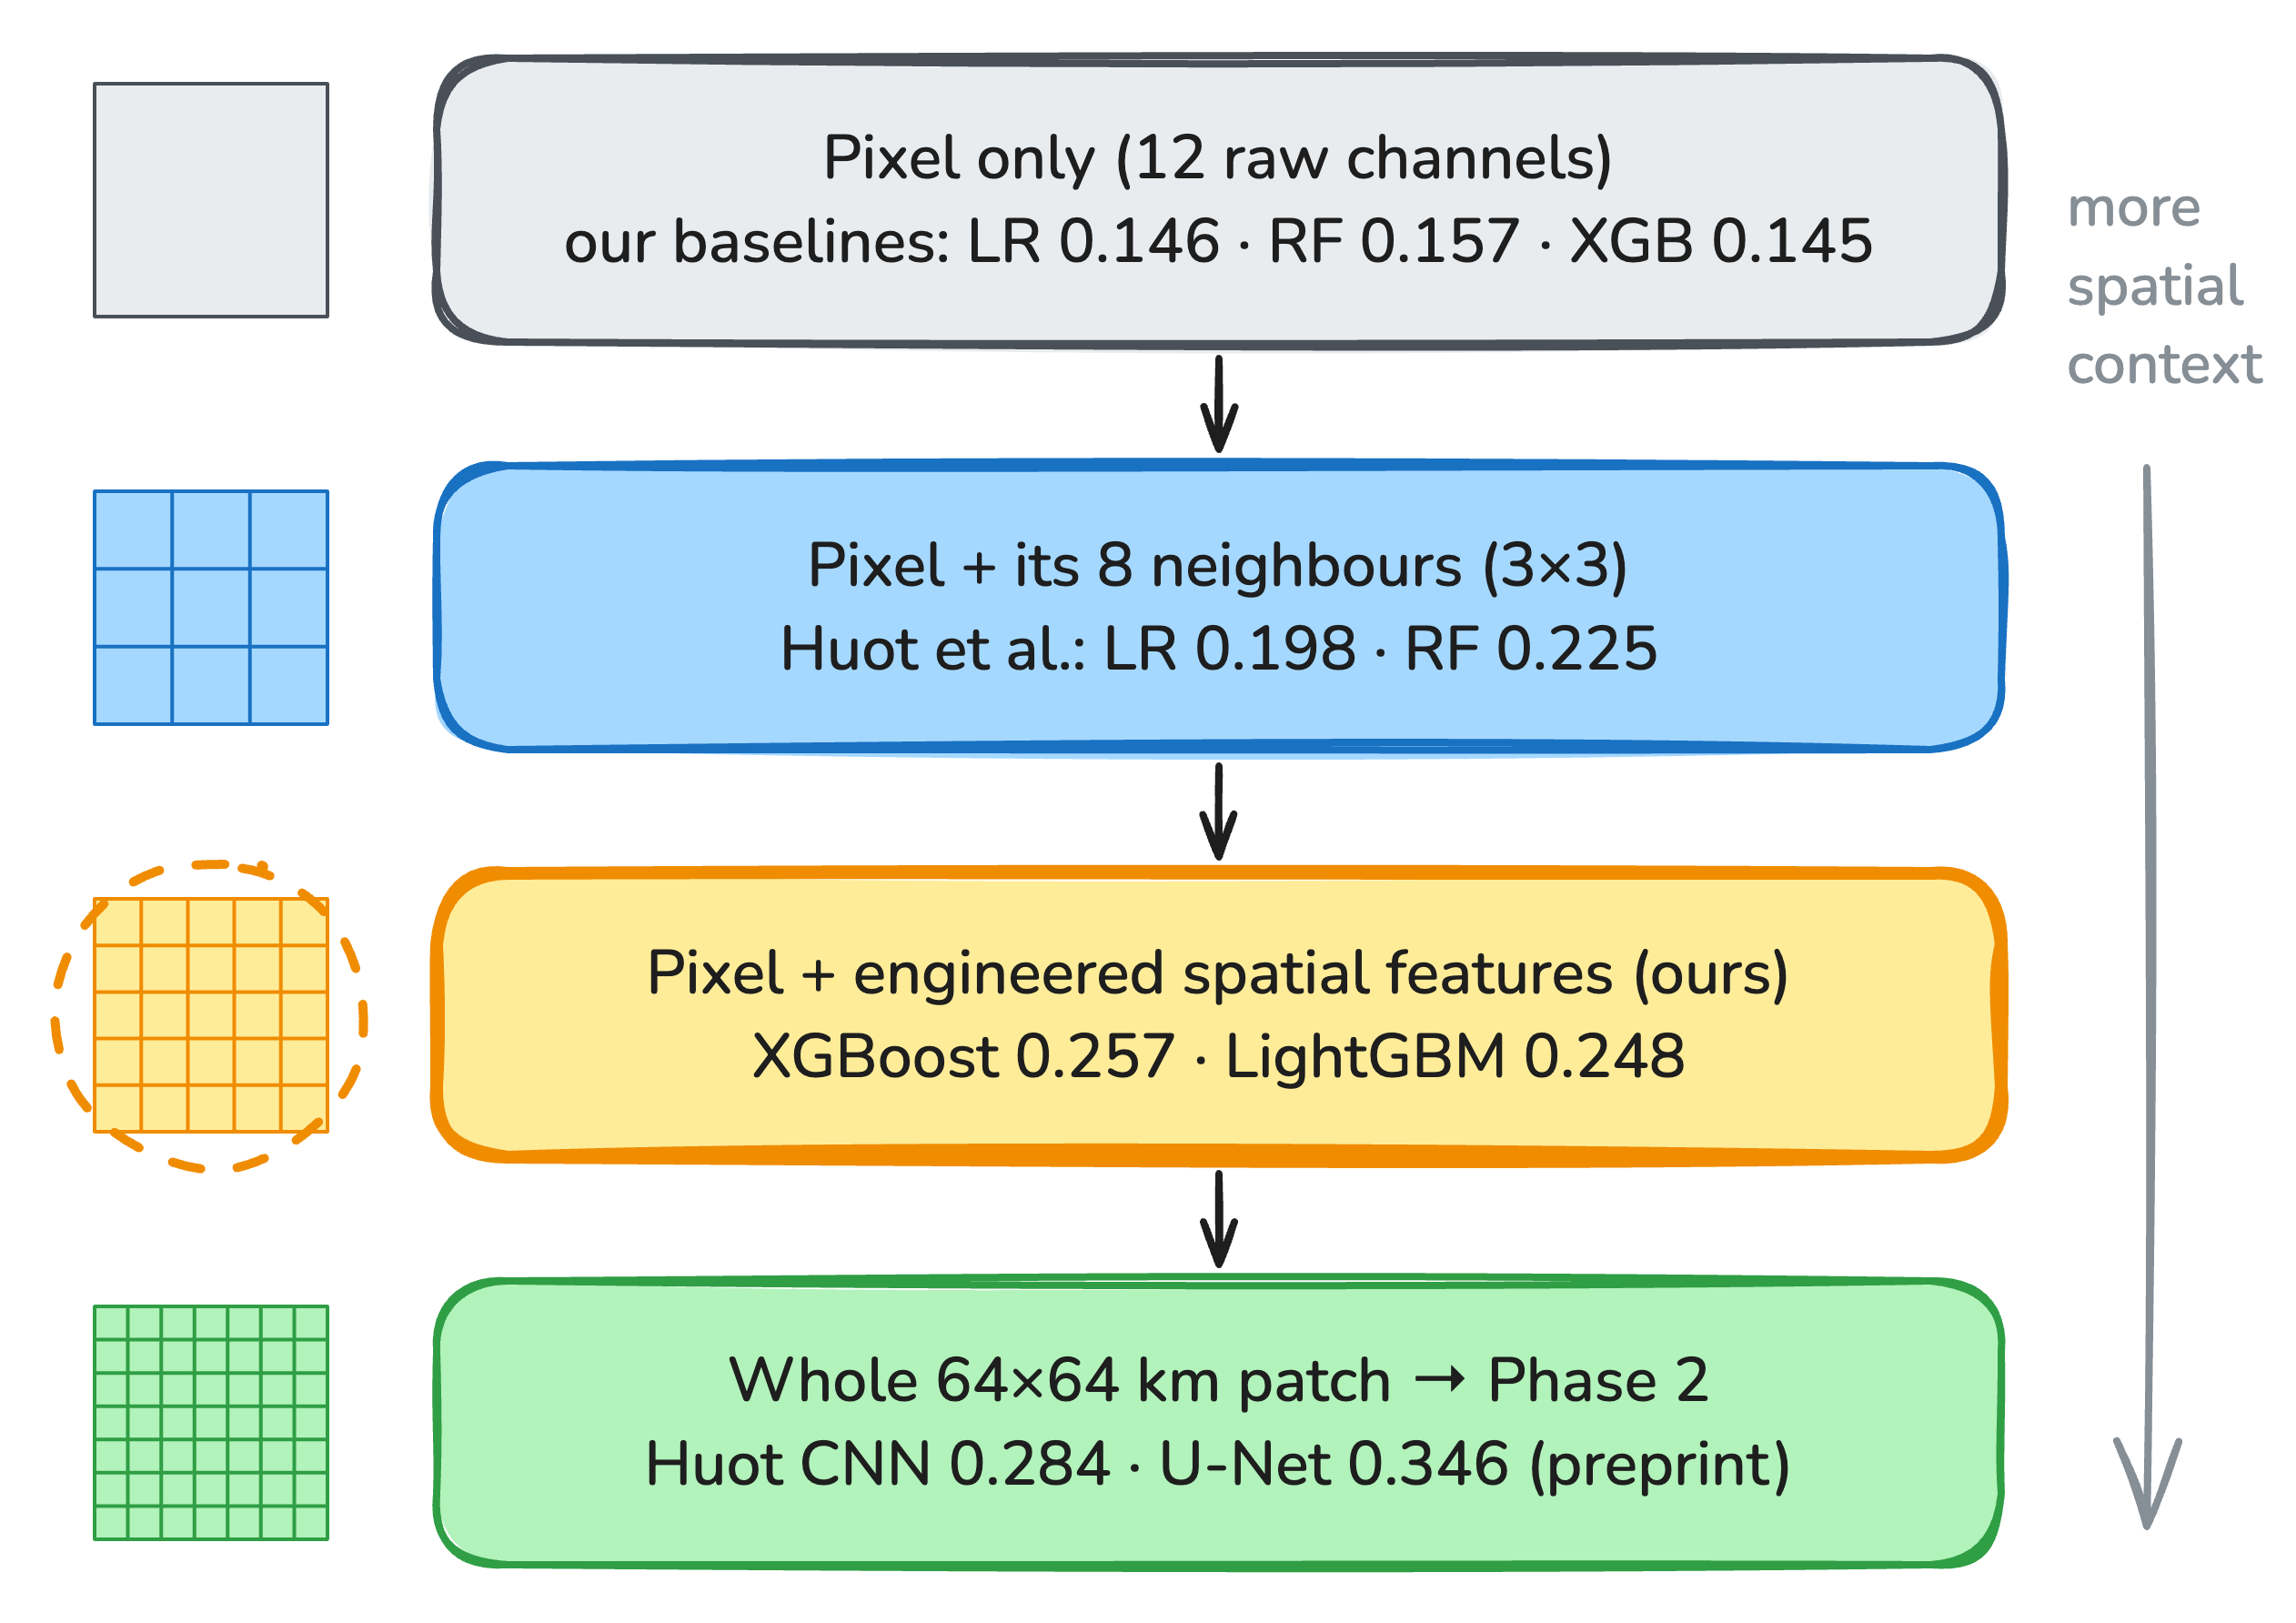
\includegraphics[width=\columnwidth]{figures/rw_context_ladder.png}
\caption{NDWS models ordered by the spatial context they see, with test PR AUC. Raw-channel baselines are
ours; the others are from~\cite{huot2022,esparza2026}.}
\label{fig:rw_ladder}
\end{figure}

% Theoretical Background (Priyanshu)
% Project numbers come from reports/best_params.json, reports/results.csv, reports/tuning_*.csv,
% reports/ablation.csv, notebooks/01_eda.ipynb, notebooks/02_evaluation.ipynb and src/*.py.
% Full derivations are in sections/appendix.tex. Uses \keyeq and projectbox from main.tex.

\section{Theoretical Background}
\label{sec:theory}

This section gives the theory behind four choices in our pipeline (Fig.~\ref{fig:pipeline}):
gradient-boosted trees, class weighting, PR AUC as the main metric, and why tuning stops helping. The
main results are stated here, and the full derivations are given in Appendix~\ref{app:derivations}.

% =============================================================================================
\subsection{Gradient boosting and second-order splits}
\label{sec:theory_gb}

Gradient boosting~\cite{friedman2001} builds a model as a sum of regression trees, adding one tree $f_m$
at a time and shrinking each by a learning rate $\eta$:
\begin{equation}
F_m(\mathbf{x}) = F_{m-1}(\mathbf{x}) + \eta\, f_m(\mathbf{x}) .
\label{eq:additive}
\end{equation}
The score $F$ is a log-odds, and the predicted probability is $p = \sigma(F) = 1/(1+e^{-F})$.
XGBoost~\cite{chen2016} chooses each tree by minimising a loss plus a penalty on tree complexity, where
$T$ is the number of leaves and $w_j$ the value of leaf $j$:
\begin{align}
\mathcal{L} &= \sum_{i=1}^{n} l(y_i, \hat{y}_i) + \sum_{k} \Omega(f_k), \label{eq:objective}\\
\Omega(f) &= \gamma T + \tfrac{1}{2}\lambda \textstyle\sum_{j} w_j^2 . \label{eq:omega}
\end{align}

\textbf{Second-order step.} At step $m$ the loss is expanded to second order around the current
prediction. With gradients $g_i$ and Hessians $h_i$ of the loss, which for log loss are
(Appendix~\ref{app:grad})
\begin{equation}
g_i = p_i - y_i, \qquad h_i = p_i(1-p_i),
\label{eq:gh}
\end{equation}
and with $G_j$ and $H_j$ the sums of $g_i$ and $h_i$ over the rows in leaf $j$, the objective becomes
one quadratic per leaf:
\begin{equation}
\mathcal{L}^{(m)} \approx \sum_{j=1}^{T} \Big[ G_j w_j + \tfrac{1}{2}(H_j + \lambda)\, w_j^2 \Big] + \gamma T .
\label{eq:leafsum}
\end{equation}

\textbf{Leaf values and split gain.} Setting the derivative with respect to $w_j$ to zero,
$G_j + (H_j+\lambda)\,w_j = 0$, gives the optimal leaf value and, substituted back, the lowest loss for
a given tree structure:
\begin{equation}
\keyeq{w_j^\ast = -\frac{G_j}{H_j + \lambda}}, \qquad
\mathcal{L}^{\ast} = -\frac{1}{2} \sum_{j=1}^{T} \frac{G_j^2}{H_j + \lambda} + \gamma T .
\label{eq:leafweight}
\end{equation}
Each leaf therefore takes one Newton step, the gradient divided by the curvature plus $\lambda$.
Splitting a leaf into a left part $L$ and a right part $R$ changes $\mathcal{L}^\ast$ by
\begin{multline}
\text{Gain} = \frac{1}{2}\left[ \frac{G_L^2}{H_L + \lambda} + \frac{G_R^2}{H_R + \lambda} \right. \\
\left. - \frac{(G_L + G_R)^2}{H_L + H_R + \lambda} \right] - \gamma .
\label{eq:gain}
\end{multline}
Trees are grown greedily, and a split is kept only if its gain is positive (Fig.~\ref{fig:th_split}).
So $\gamma$ is the minimum loss reduction that pays for a new leaf, and $\lambda$ shrinks leaf values
toward zero, most strongly in leaves with a small Hessian sum.

\begin{figure}[t]
\centering
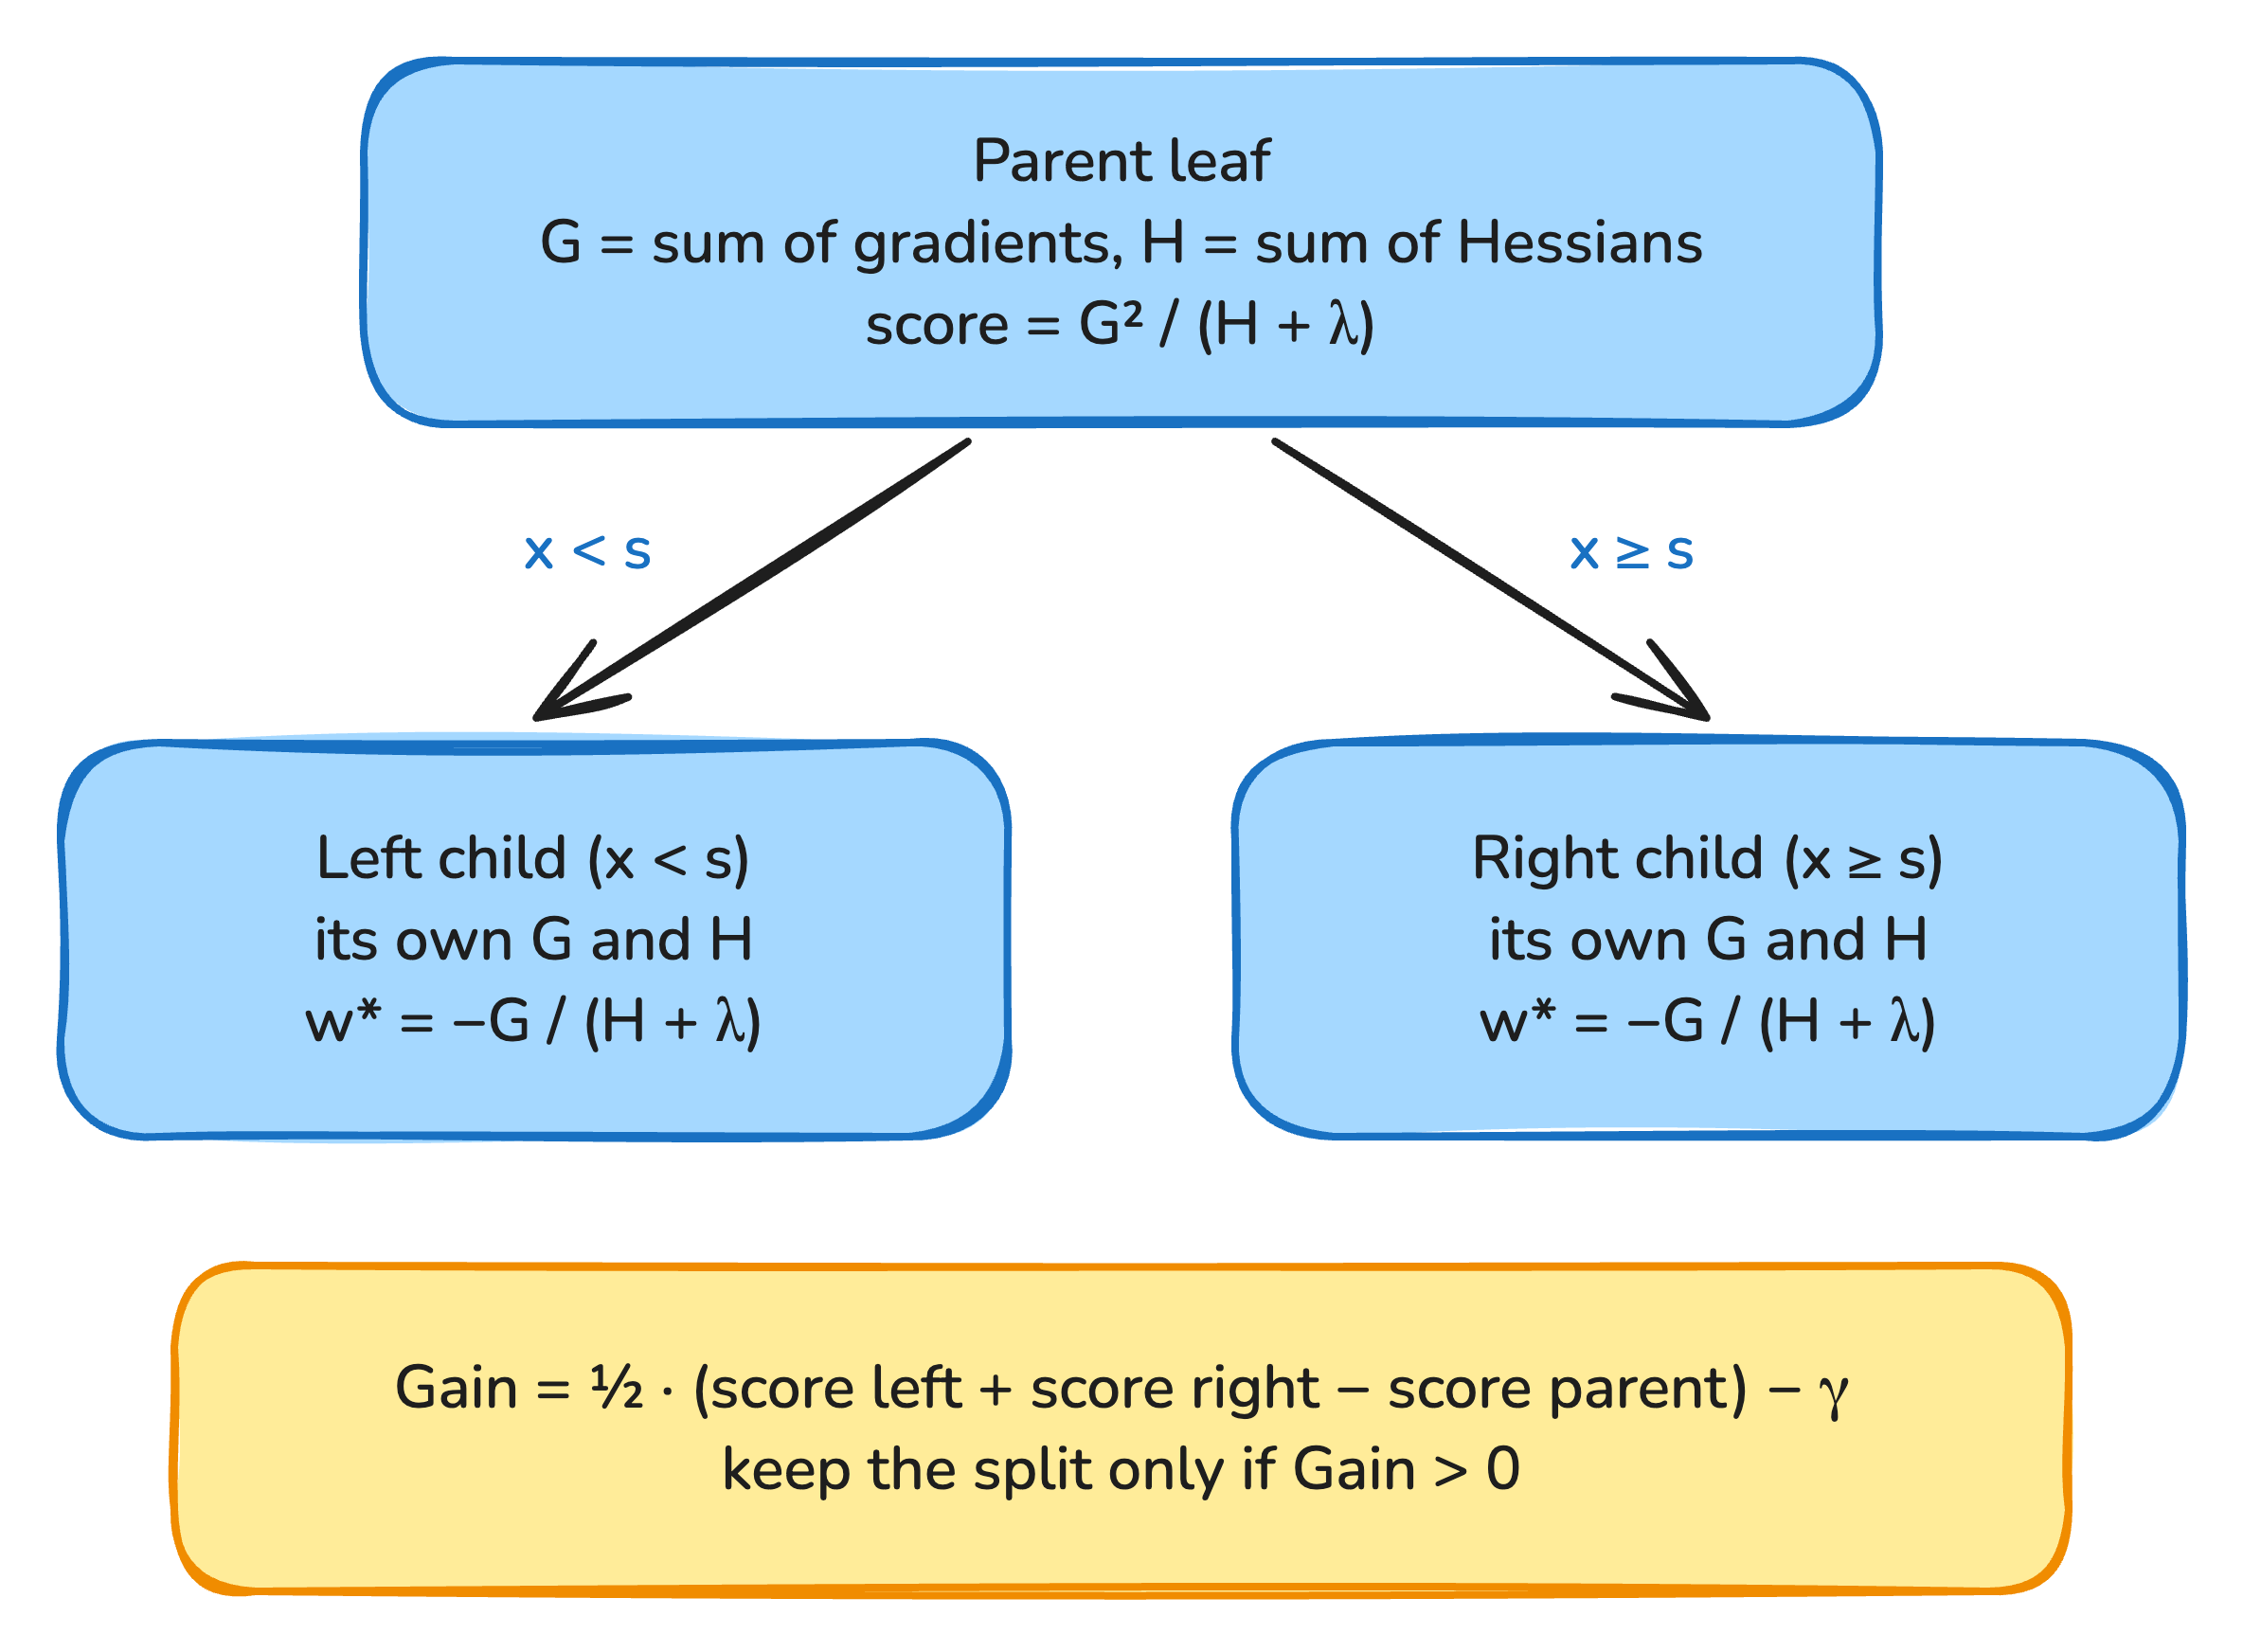
\includegraphics[width=0.92\columnwidth]{figures/th_split.png}
\caption{One split in XGBoost. Each child gets the value $w^\ast$ of (\ref{eq:leafweight}); the split is
kept only if the gain (\ref{eq:gain}) is positive.}
\label{fig:th_split}
\end{figure}

\textbf{LightGBM.} LightGBM~\cite{ke2017} minimises the same kind of objective but differs in four ways.
It bins each feature into a histogram, so split search scans bins instead of sorted values. It grows
trees leaf-wise, always splitting the leaf with the largest loss reduction, so tree size is set by
\texttt{num\_leaves} rather than depth. It can sample rows by gradient size (GOSS). It bundles sparse
features that are rarely non-zero together (EFB).

\textbf{Early stopping.} Each added tree lowers the training loss, so the number of trees sets how
closely the ensemble fits the training table. Stopping when the held-out score no longer improves
chooses that number on data the trees were not fitted to, and in that way limits overfitting.

\begin{projectbox}
Table~\ref{tab:hyper} maps each symbol to its parameter and selected value (search space in
Table~\ref{tab:space}). In XGBoost, \texttt{min\_child\_weight} is the smallest $H_j$ allowed in a child.
By (\ref{eq:gh}) a no-fire row has $h \le 0.25$ and a fire row, weighted by 5, has $h \le 1.25$, so our
value of 1 is a weak constraint. The other two penalties are strong: $\gamma = 1$ is the largest value
searched, and $\lambda = 7.22$ lies near the top of $[0.1, 10]$. XGBoost uses histogram binning
(\texttt{tree\_method=hist}). LightGBM grows leaf-wise with 15 leaves and uses plain bagging, not GOSS.
Both models stop after 50 rounds without improvement in eval PR AUC, keeping 216 and 294 of at most
1\,000 trees. We stop on PR AUC rather than log loss because the 1:5 training table shifts the
probabilities (Section~\ref{sec:theory_imb}). On log loss, our LightGBM runs stopped after a single tree
(\texttt{src/train.py}).
\end{projectbox}

\begin{table}[t]
\centering
\caption{Boosting symbols and our selected values (\texttt{reports/best\_params.json}).}
\label{tab:hyper}
\small
\setlength{\tabcolsep}{4pt}
\renewcommand{\arraystretch}{1.12}
\begin{tabular}{l>{\raggedright\arraybackslash}p{2.75cm}rr}
\toprule
\rowcolor{tblhead}
\textbf{Symbol} & \textbf{Meaning} & \textbf{XGBoost} & \textbf{LightGBM} \\
\midrule
$\lambda$ & L2 penalty on leaf values & 7.22 & 0.28 \\
$\gamma$ & minimum gain per split & 1 & 1 \\
$\eta$ & learning rate & 0.026 & 0.058 \\
$\min H_j$ & minimum leaf size & $H_j \ge 1$ & 500 rows \\
- & tree size & depth 6 & 15 leaves \\
- & rows per tree & 0.73 & 0.98 \\
- & features per tree & 0.63 & 0.88 \\
$w$ & weight on fire rows & 5.0 & 5.0 \\
$M$ & trees after early stopping & 216 & 294 \\
\bottomrule
\end{tabular}
\end{table}

% =============================================================================================
\subsection{Class imbalance and class weighting}
\label{sec:theory_imb}

Next-day fire covers 1.10\% of labelled training pixels, about 90 no-fire pixels per fire pixel. Left
uncorrected, no-fire rows dominate $G_j$ and $H_j$ in every leaf. The two standard corrections are to
subsample negatives and to weight positives.

\textbf{Weighting acts like duplication.} With weight $w$ on positives, the log loss and the gradient and
Hessian of a positive row become (Appendix~\ref{app:grad})
\begin{gather}
l_w = -\big[\, w\, y \log p + (1 - y) \log(1-p) \,\big], \label{eq:weighted_ll}\\
g_i = w\,(p_i - 1), \qquad h_i = w\,p_i(1-p_i). \label{eq:weighted_gh}
\end{gather}
Both are $w$ times their unweighted values. Trees see the data only through $G$ and $H$, so a weighted
positive acts exactly like $w$ copies of the same row.

\textbf{Both corrections shift the probabilities.} Keeping a share $r$ of the negatives and weighting
positives by $w$ changes the class prior seen by the loss but not the feature distribution within each
class. By Bayes' rule (Appendix~\ref{app:shift}), the probability $p'$ learned in training and the true
probability $p$ differ by a constant factor in their odds:
\begin{equation}
\keyeq{\frac{p'}{1-p'} = \frac{w}{r}\cdot\frac{p}{1-p}}
\label{eq:prior_shift}
\end{equation}
Solving for $p$ maps a model score back to the true scale:
\begin{equation}
p = \frac{p'}{p' + (w/r)(1-p')} .
\label{eq:inverse_shift}
\end{equation}
The map is strictly increasing, so the order of pixels is unchanged. Ranking metrics (PR AUC, ROC AUC,
recall at a fixed FPR) are unaffected, but a fixed threshold must be chosen on data with the true class
ratio.

\textbf{Focal loss.} Lin et al.~\cite{lin2017} reshape the loss instead of the data. With $p_t = p$ for
positives and $1-p$ for negatives,
\begin{equation}
\mathrm{FL}(p_t) = -\alpha_t (1 - p_t)^{\gamma_f} \log p_t ,
\label{eq:focal}
\end{equation}
where $\gamma_f = 2$ and $\alpha = 0.25$ worked best in their experiments. The factor $(1-p_t)^{\gamma_f}$
is close to zero for well-classified rows, so easy negatives contribute little. With $\gamma_f = 0$ the
loss reduces to (\ref{eq:weighted_ll}).

\begin{figure}[t]
\centering
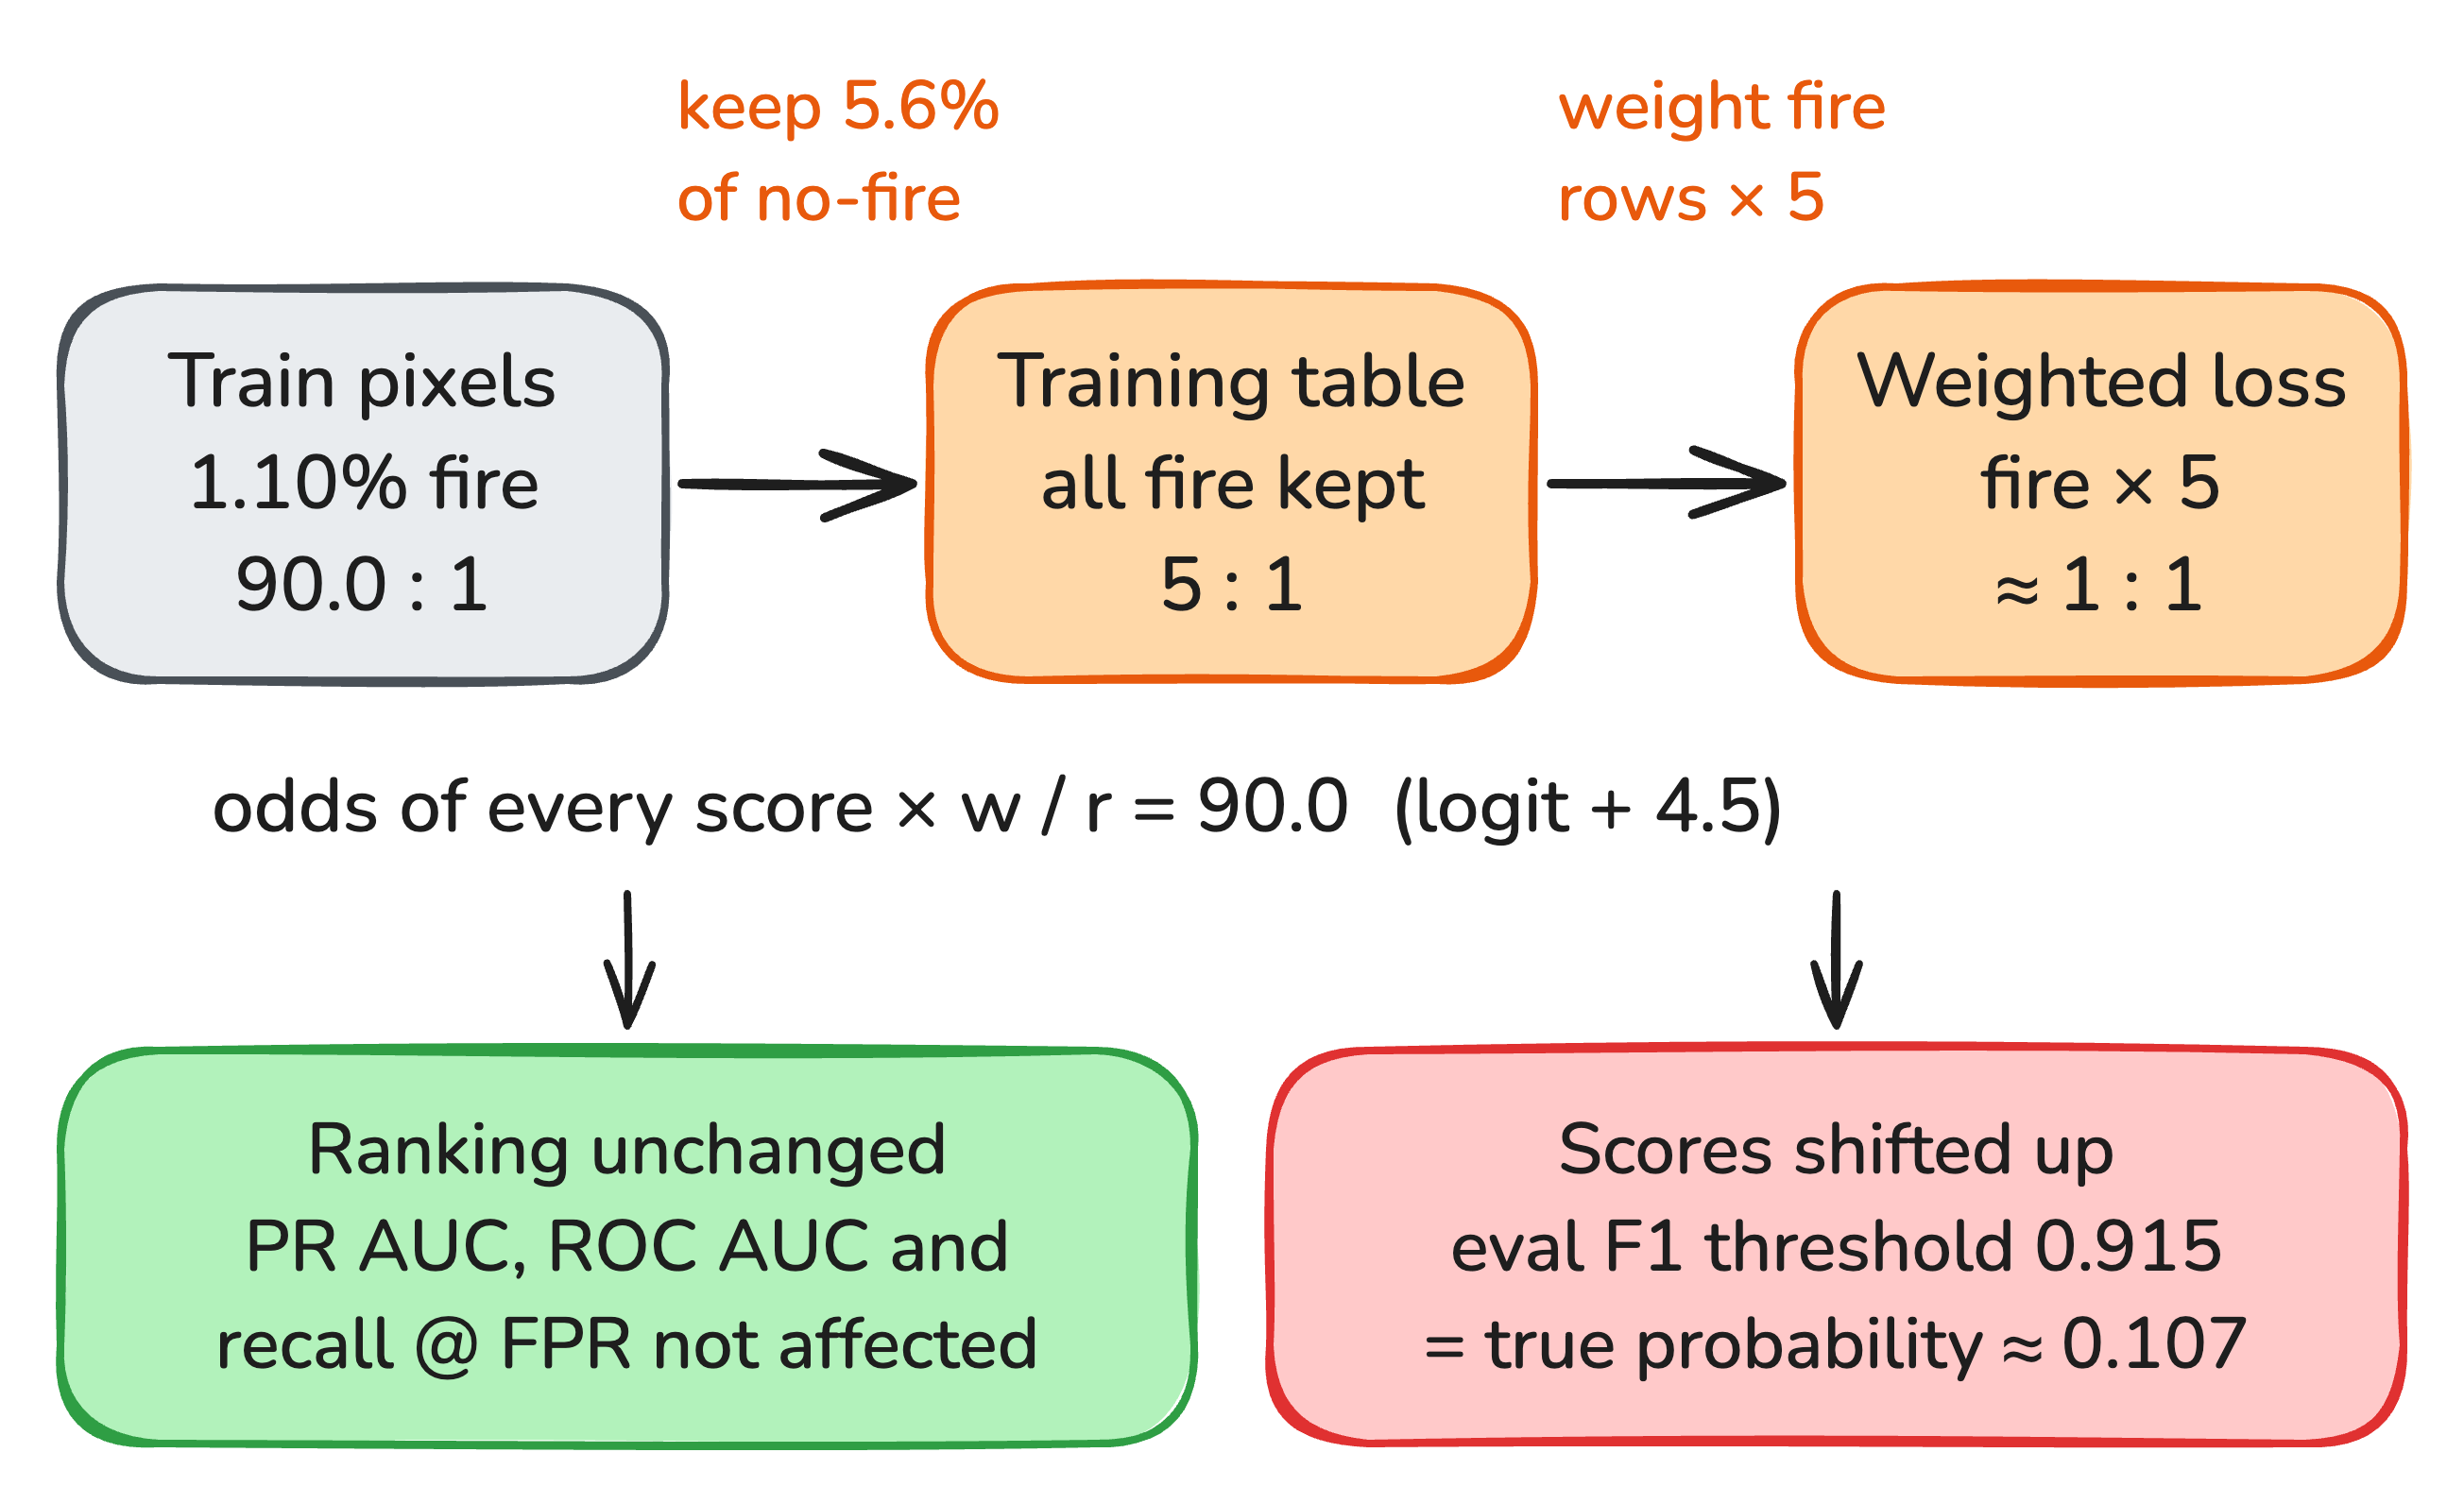
\includegraphics[width=\columnwidth]{figures/th_imbalance.png}
\caption{Subsampling and weighting turn a 90:1 problem into a balanced one and shift every score, by
(\ref{eq:prior_shift}).}
\label{fig:th_imbalance}
\end{figure}

\begin{figure}[t]
\centering
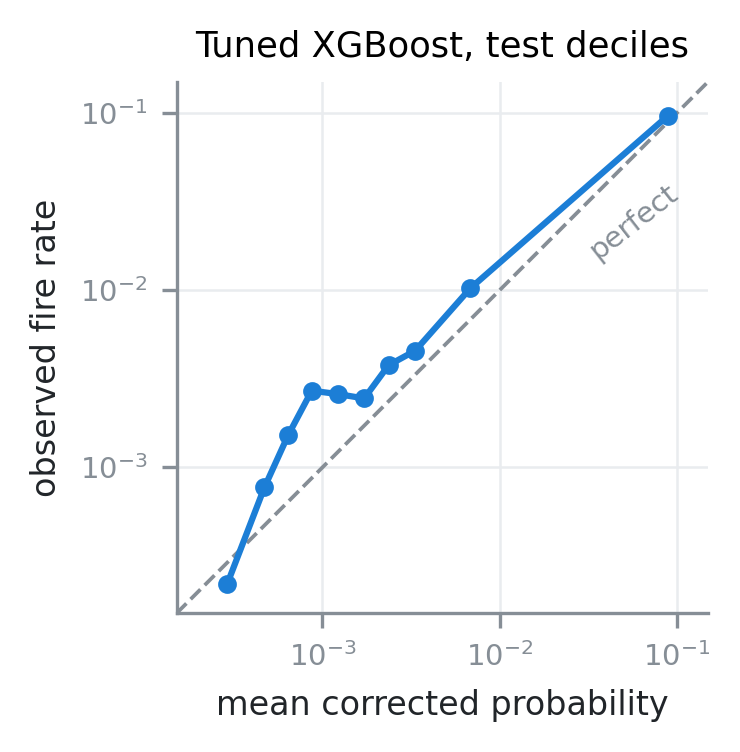
\includegraphics[width=0.68\columnwidth]{figures/th_calibration.png}
\caption{Calibration of the tuned XGBoost on test after undoing the prior shift with
(\ref{eq:inverse_shift}). Each point is one tenth of the test pixels, ordered by score; log scales.}
\label{fig:th_calibration}
\end{figure}

\begin{projectbox}
The training table keeps every fire pixel and 5 no-fire pixels per fire pixel, so $r = 5/90.0 = 0.056$,
and fire rows get $w = 5$ (\texttt{scale\_pos\_weight}). The odds are therefore multiplied by
$w/r = 90.0$, and the model trains as if the classes were balanced (Fig.~\ref{fig:th_imbalance}). This
explains the high F1 threshold of 0.915 chosen on eval: by (\ref{eq:inverse_shift}) it corresponds to a
probability of 0.107 on the true scale, while a score of 0.5 corresponds to 0.011, the training fire
rate. We checked the correction on test with a retrained copy of the model (Appendix~\ref{app:checks}).
After (\ref{eq:inverse_shift}), the mean probability is 0.0107 against an observed fire rate of 0.0125,
and in the top score decile 0.089 against 0.097 (Fig.~\ref{fig:th_calibration}). The corrected values
are therefore close to true risk and slightly low. Most of the overall gap matches the higher fire rate
of test (1.25\% against 1.10\% in train); below a corrected value of about 0.002 they are up to about 3 times
too low.

We did not use focal loss, because the boosting libraries would need it as a custom objective and weighting
already balances the loss. It is a candidate for Phase~2, where a segmentation network computes its loss
on every pixel of a patch (Huot et al.\ use a weight of 3 on fire for their CNN~\cite{huot2022}).
\end{projectbox}

% =============================================================================================
\subsection{PR AUC versus ROC AUC under imbalance}
\label{sec:theory_pr}

With $P$ fire and $N$ no-fire pixels, and TP and FP the true and false positives at a threshold,
\begin{align}
\mathrm{TPR} &= \frac{\mathrm{TP}}{P}, \qquad \mathrm{FPR} = \frac{\mathrm{FP}}{N}, \label{eq:rates}\\
\mathrm{Precision} &= \frac{\mathrm{TP}}{\mathrm{TP} + \mathrm{FP}} . \label{eq:prec_def}
\end{align}
The ROC curve plots TPR (recall) against FPR, and the PR curve plots precision against recall. Writing
precision in terms of the two rates and the prevalence $\pi = P/(P+N)$ (Appendix~\ref{app:prec}) gives
\begin{equation}
\keyeq{\mathrm{Precision} = \frac{\pi\,\mathrm{TPR}}{\pi\,\mathrm{TPR} + (1 - \pi)\,\mathrm{FPR}}}
\label{eq:precision}
\end{equation}
TPR and FPR are each computed within one class, so the ROC curve does not depend on $\pi$. Precision does:
when $\pi$ is small, $(1-\pi)\,\mathrm{FPR}$ dominates the denominator even at a small FPR.

A random classifier has ROC AUC 0.5 at any imbalance, but it also has $\mathrm{TPR} = \mathrm{FPR}$, so by
(\ref{eq:precision}) its precision is $\pi$ everywhere and its PR AUC equals the
prevalence~\cite{saito2015}. We compute PR AUC as average precision,
$\mathrm{AP} = \sum_k (R_k - R_{k-1})\, P_k$, a step sum over thresholds with recall $R_k$ and precision
$P_k$. Davis and Goadrich~\cite{davis2006} prove that a curve dominates in ROC space if and only if it
dominates in PR space, and that linear interpolation is wrong in PR space, which is why AP uses a step
sum. Saito and Rehmsmeier~\cite{saito2015} show that on imbalanced data the ROC plot can be deceptive,
while the PR plot is not.

\begin{figure}[t]
\centering
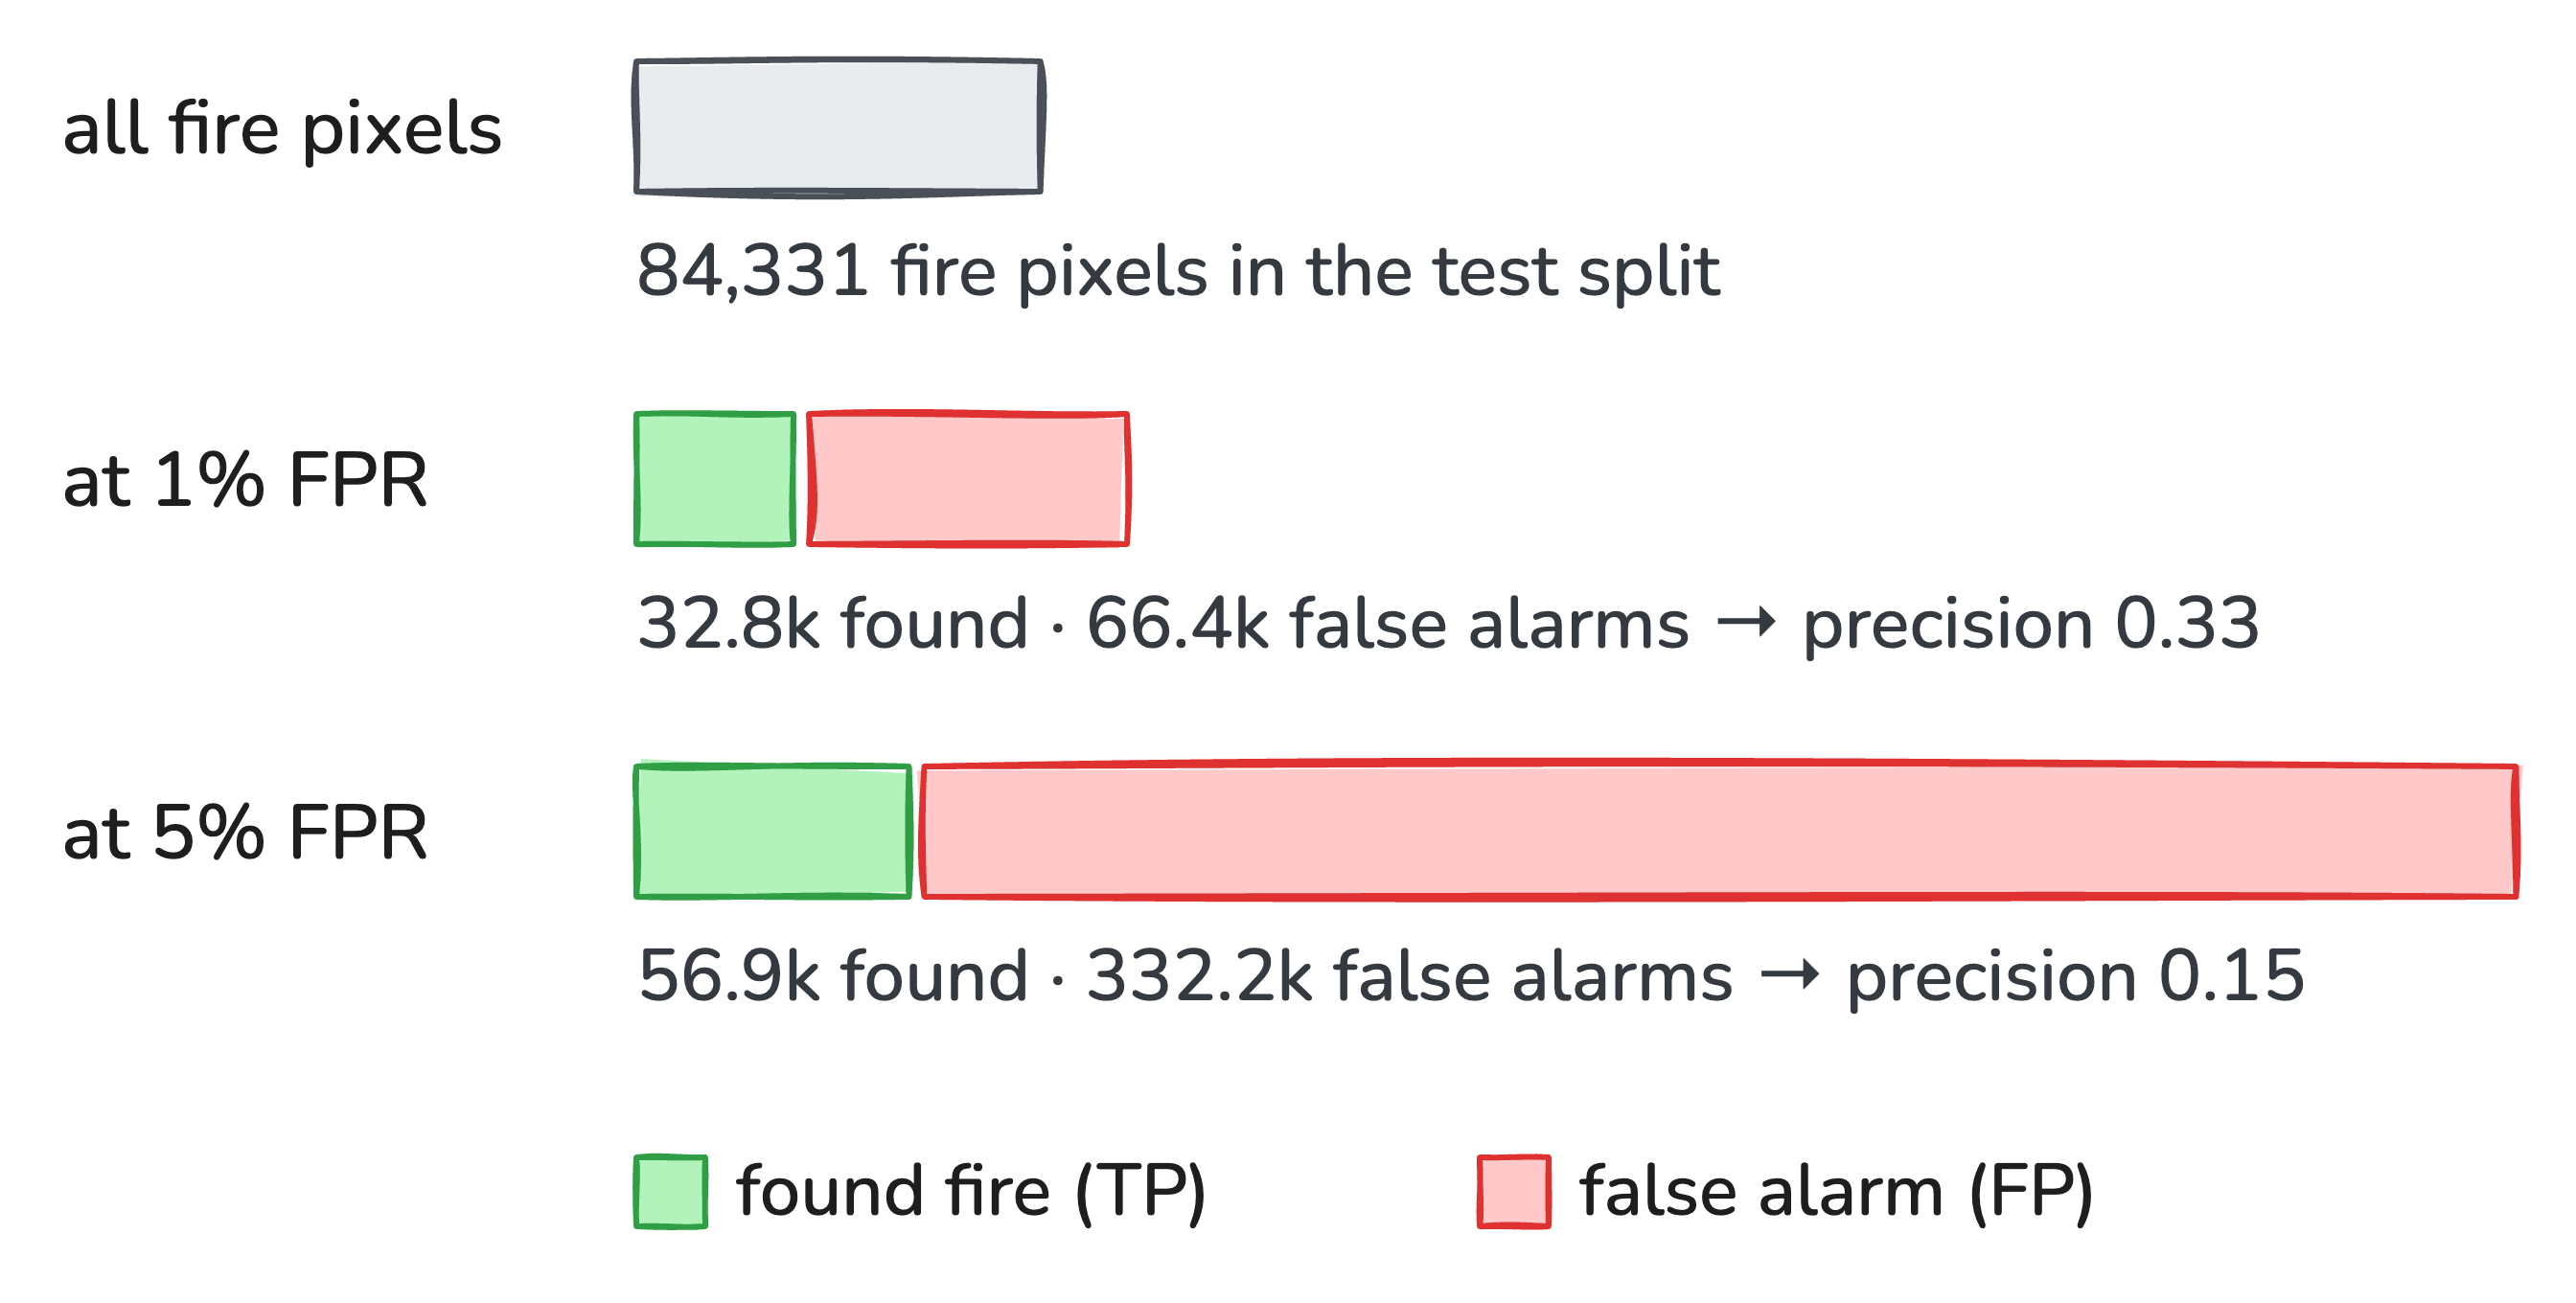
\includegraphics[width=\columnwidth]{figures/th_false_alarms.png}
\caption{Tuned XGBoost on the test split at 1\% and 5\% FPR. Box widths are proportional to pixel counts.}
\label{fig:th_false_alarms}
\end{figure}

\begin{projectbox}
Fire is 1.25\% of labelled test pixels, so a random model scores PR AUC 0.0125. Our tuned XGBoost scores
ROC AUC 0.906 but PR AUC 0.257 (Table~\ref{tab:results}). Fig.~\ref{fig:th_false_alarms} shows why the
two differ. At 1\% FPR the model finds about 32\,800 of the 84\,331 fire pixels but raises about 66\,400
false alarms, so precision is 0.33. At 5\% FPR it finds about 56\,900 against 332\,200 false alarms, a
precision of 0.15. Recall at 1\% and 5\% FPR therefore fixes the false-alarm budget an operator would
have to check. Precision, recall and F1 use the F1-optimal threshold from eval, applied unchanged to test.
Choosing it on test would overstate F1 (0.358 against 0.332).
\end{projectbox}

% =============================================================================================
\subsection{Bias-variance trade-off of tree ensembles}
\label{sec:theory_bv}

For squared loss, the expected error of a model $\hat{f}$ trained on a random training set splits into
three parts, where $f$ is the true function and $\sigma^2$ the noise variance:
\begin{equation}
\mathbb{E}\big[(y - \hat{f})^2\big] =
\underbrace{\big(\mathbb{E}\hat{f} - f\big)^2}_{\text{bias}^2}
+ \underbrace{\mathrm{Var}\,\hat{f}}_{\text{variance}}
+ \underbrace{\sigma^2}_{\text{noise}} .
\label{eq:biasvar}
\end{equation}
For log loss the split is not exactly additive, but the same reasoning applies. Bias comes from a model or
input representation that is too restricted, and variance from sensitivity to the training sample.

\textbf{Averaging trees.} For $B$ trees, each with variance $\sigma^2$ and pairwise correlation $\rho$, the
variance of their average is (Appendix~\ref{app:var})
\begin{equation}
\keyeq{\mathrm{Var}\Big(\frac{1}{B}\sum_{b=1}^{B} \hat{f}_b\Big) = \rho\,\sigma^2 + \frac{1-\rho}{B}\,\sigma^2}
\label{eq:rf_var}
\end{equation}
More trees remove only the second term, so the shared variance $\rho\sigma^2$ stays. Random
forests~\cite{breiman2001} lower $\rho$ with bootstrap samples and a random subset of features at each
split.

\textbf{Boosting.} Boosting starts from small, high-bias trees and lowers the bias step by step. Its
variance is held back by shrinkage, early stopping, tree size, minimum leaf size, the penalties $\lambda$
and $\gamma$, and row and column subsampling, which by (\ref{eq:rf_var}) also make the trees less alike.

\begin{projectbox}
Across 20 random XGBoost configurations (depth 4 to 10, learning rate 0.023 to 0.28), eval PR AUC stayed
between 0.196 and 0.207, and the 20 LightGBM configurations between 0.189 and 0.203. The settings that
trade bias against variance therefore move the score by only about 0.01. Changing the inputs moves it far
more: with the same hyperparameters, removing the fire-neighbourhood features lowers LightGBM's test PR
AUC from 0.248 to 0.048 (Table~\ref{tab:ablation}).

Learning curves (Fig.~\ref{fig:th_learning}) show where the remaining error lies. Trained on 5\% of the
training patches (0.2M rows) instead of all of them (3.9M rows), the tuned XGBoost reaches almost the
same eval PR AUC (0.204 against 0.207), and eval ROC AUC stays between 0.891 and 0.900. More data
narrows the train-eval gap in ROC AUC from 0.080 to 0.055 only by lowering the training score. More trees
do the opposite: training ROC AUC keeps rising while eval peaks at 0.898 near 270 trees and falls to
0.883 at 1000, the variance that early stopping (216 trees) avoids. An eval score that does not move with
20 times more data means the model is not limited by variance. What remains is bias from the input
representation, since each pixel sees the patch only through fixed-radius summaries, and noise the inputs
cannot explain, such as which fires will die down. This is why Phase~2 moves to a spatial model rather
than to more data or tuning.
\end{projectbox}

\begin{figure}[t]
\centering
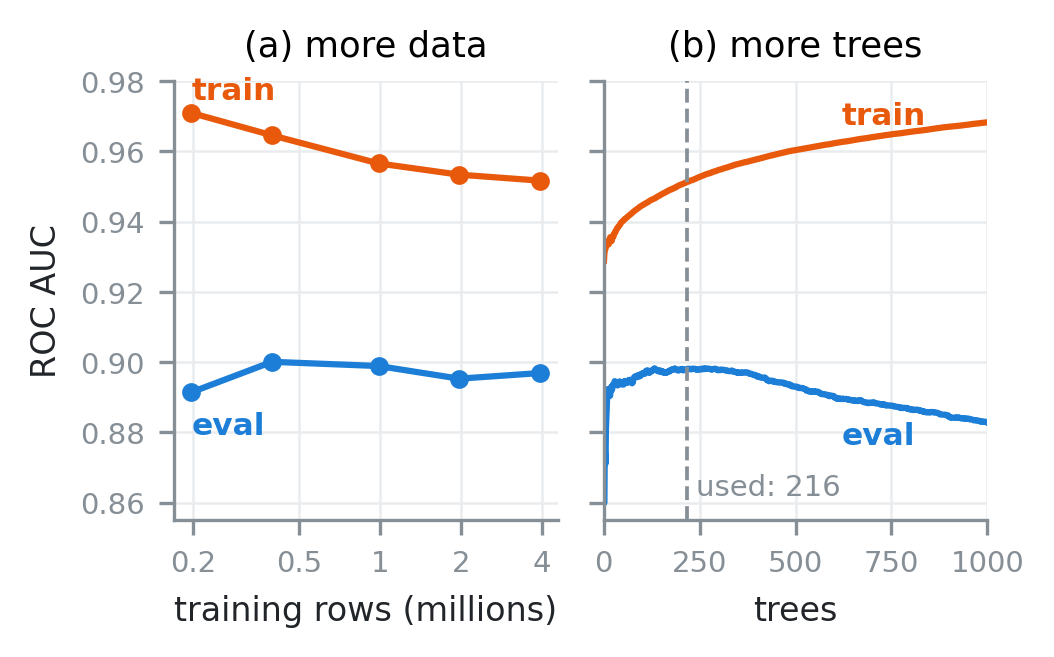
\includegraphics[width=\columnwidth]{figures/th_learning_curves.png}
\caption{Tuned XGBoost, ROC AUC on training rows and on eval. (a) Trained on 5--100\% of the training
patches. (b) Trees added without early stopping; dashed: the 216 trees used. ROC AUC is shown because the
training table is subsampled 1:5, which changes PR AUC but not ROC AUC (Section~\ref{sec:theory_pr}).}
\label{fig:th_learning}
\end{figure}

% Dataset and EDA, with the feature-group ablation
% Refers to tab:clip and tab:features from the Methodology section.

\section{Dataset and Exploratory Analysis}

\subsection{Dataset}
We use the Next Day Wildfire Spread dataset~\cite{huot2022}: 18\,545 samples of active fires across
the contiguous United States from 2012 to 2020. Each sample is a $64\times64$\,km patch at 1\,km
resolution with 12 input channels on day $t$ (elevation from SRTM; wind direction and speed, minimum
and maximum temperature, specific humidity, precipitation and ERC from GRIDMET; the Palmer drought
index from GRIDMET Drought; NDVI from VIIRS; population density from GPWv4; and the MODIS active-fire
mask) and the MODIS fire mask on day $t+1$ as the label. Fires more than 10\,km apart are treated as
separate events, and every sample contains fire on day $t$. Calendar weeks are assigned at random
to train, eval and test in an 8:1:1 ratio with a one-day buffer, giving 14\,979 / 1\,877 / 1\,689 patches.

\subsection{Labels and class imbalance}
Fire masks use three values: fire (1), no fire (0) and uncertain ($-1$, e.g.\ cloud or smoke).
Uncertain pixels make up 1.1--1.4\% of day-$t$ masks and 2.3--2.8\% of day-$t{+}1$ masks, with
similar shares in every split, so ignoring them in training and evaluation introduces no shift
between splits. Next-day fire covers only 1.10\% of labelled training pixels (90:1), 1.37\% on eval
and 1.25\% on test; an all-zero predictor would exceed 98.7\% accuracy, which is why we report
PR AUC. Across the 14\,979 training patches, 58.2\% of fires grow from day $t$ to $t+1$, 38.7\% shrink and 3.1\% keep
the same size (Fig.~\ref{fig:growth}), matching the 58\%/39\% reported by Huot et al.
Shrinking fires make persistence over-predict, and many small day-$t$ fires gain far more pixels
on day $t+1$.

\begin{figure}[t]
\centering
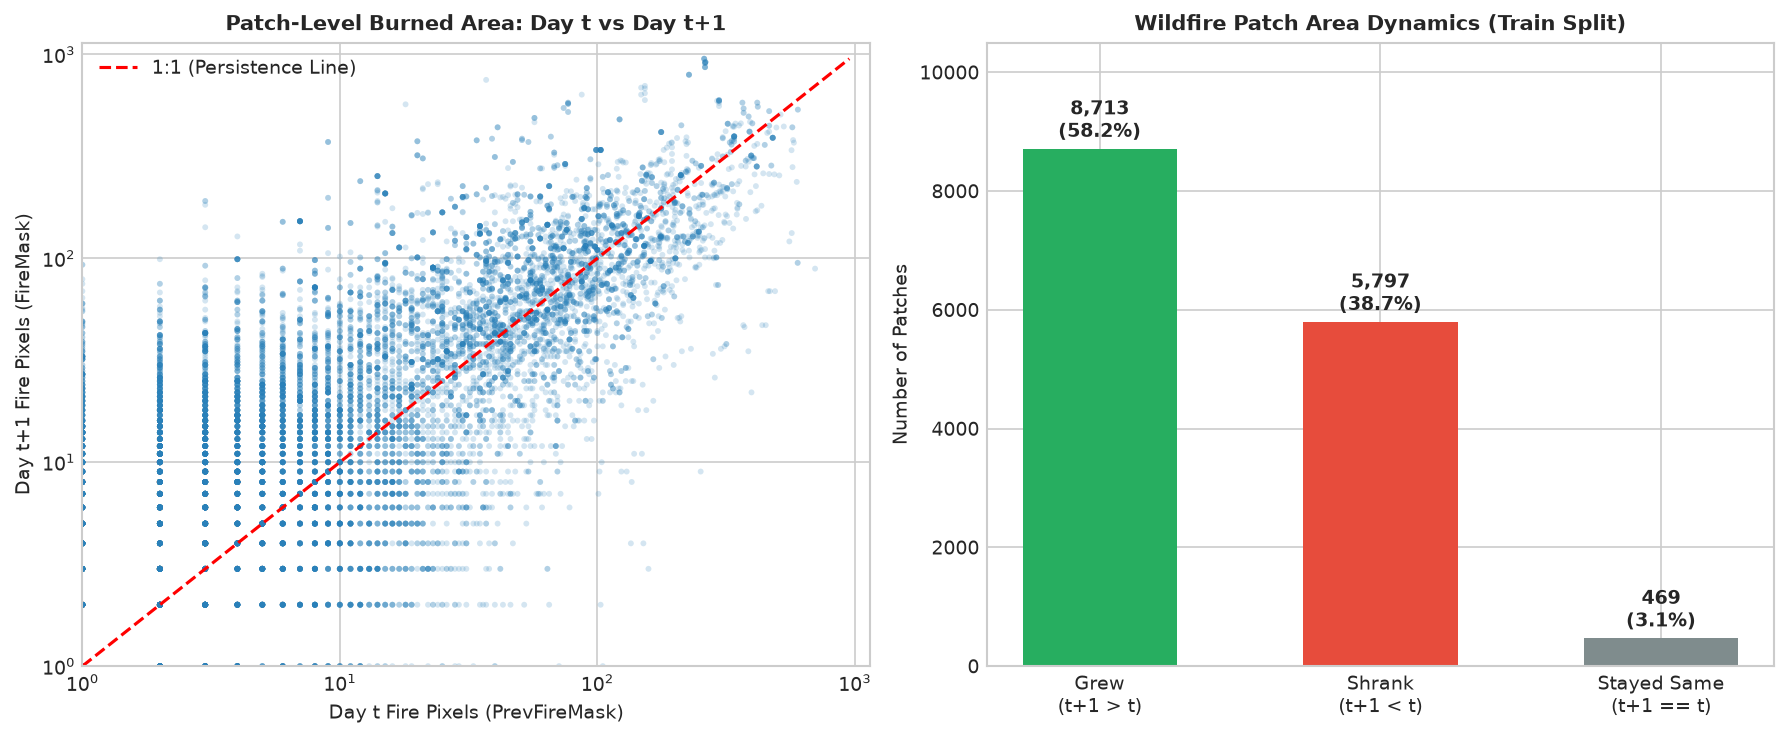
\includegraphics[width=\columnwidth]{figures/eda_patch_fire_growth.png}
\caption{Burned area per training patch on day $t$ vs.\ day $t+1$ (left, log scale, dashed line =
persistence) and the share of patches that grow, shrink or stay the same (right).}
\label{fig:growth}
\end{figure}

\subsection{Data quality}
The raw export contains physically impossible values: wind direction outside $[0^\circ, 360^\circ]$
in 0.23\% of training pixels (from $-505\,870^\circ$ to $37\,736^\circ$), temperatures from $-445$\,K
to 1\,230\,K in 0.36\% of pixels, negative precipitation in 9.8\% of pixels, and a few negative
wind speed, humidity and ERC values. These are corrected as described in the Methodology section
(Table~\ref{tab:clip}). Negative elevation (down to $-45$\,m) and negative NDVI (water, snow) are
real and left unchanged. NDVI is stored multiplied by $10^4$.

\subsection{Channel relationships and marginal signal}
Minimum and maximum temperature are strongly correlated (Spearman $\rho = 0.89$), humidity follows
temperature ($\rho = 0.70$ with \texttt{tmmn}), and elevation correlates with ERC ($0.66$) and
negatively with humidity ($-0.48$) and population ($-0.47$). The day-$t$ fire mask has near-zero rank
correlation with every raw channel ($|\rho| \le 0.09$). Comparing next-day fire and no-fire pixels
(balanced sample, Fig.~\ref{fig:fire_vs_nofire}), ERC (median 75 vs.\ 54) and elevation (1\,414 vs.\
709\,m) separate the classes most clearly, maximum temperature and NDVI shift slightly (28.0 vs.\
26.8\,$^\circ$C; 0.51 vs.\ 0.55), and wind speed and specific humidity barely differ at the median.

\begin{figure}[t]
\centering
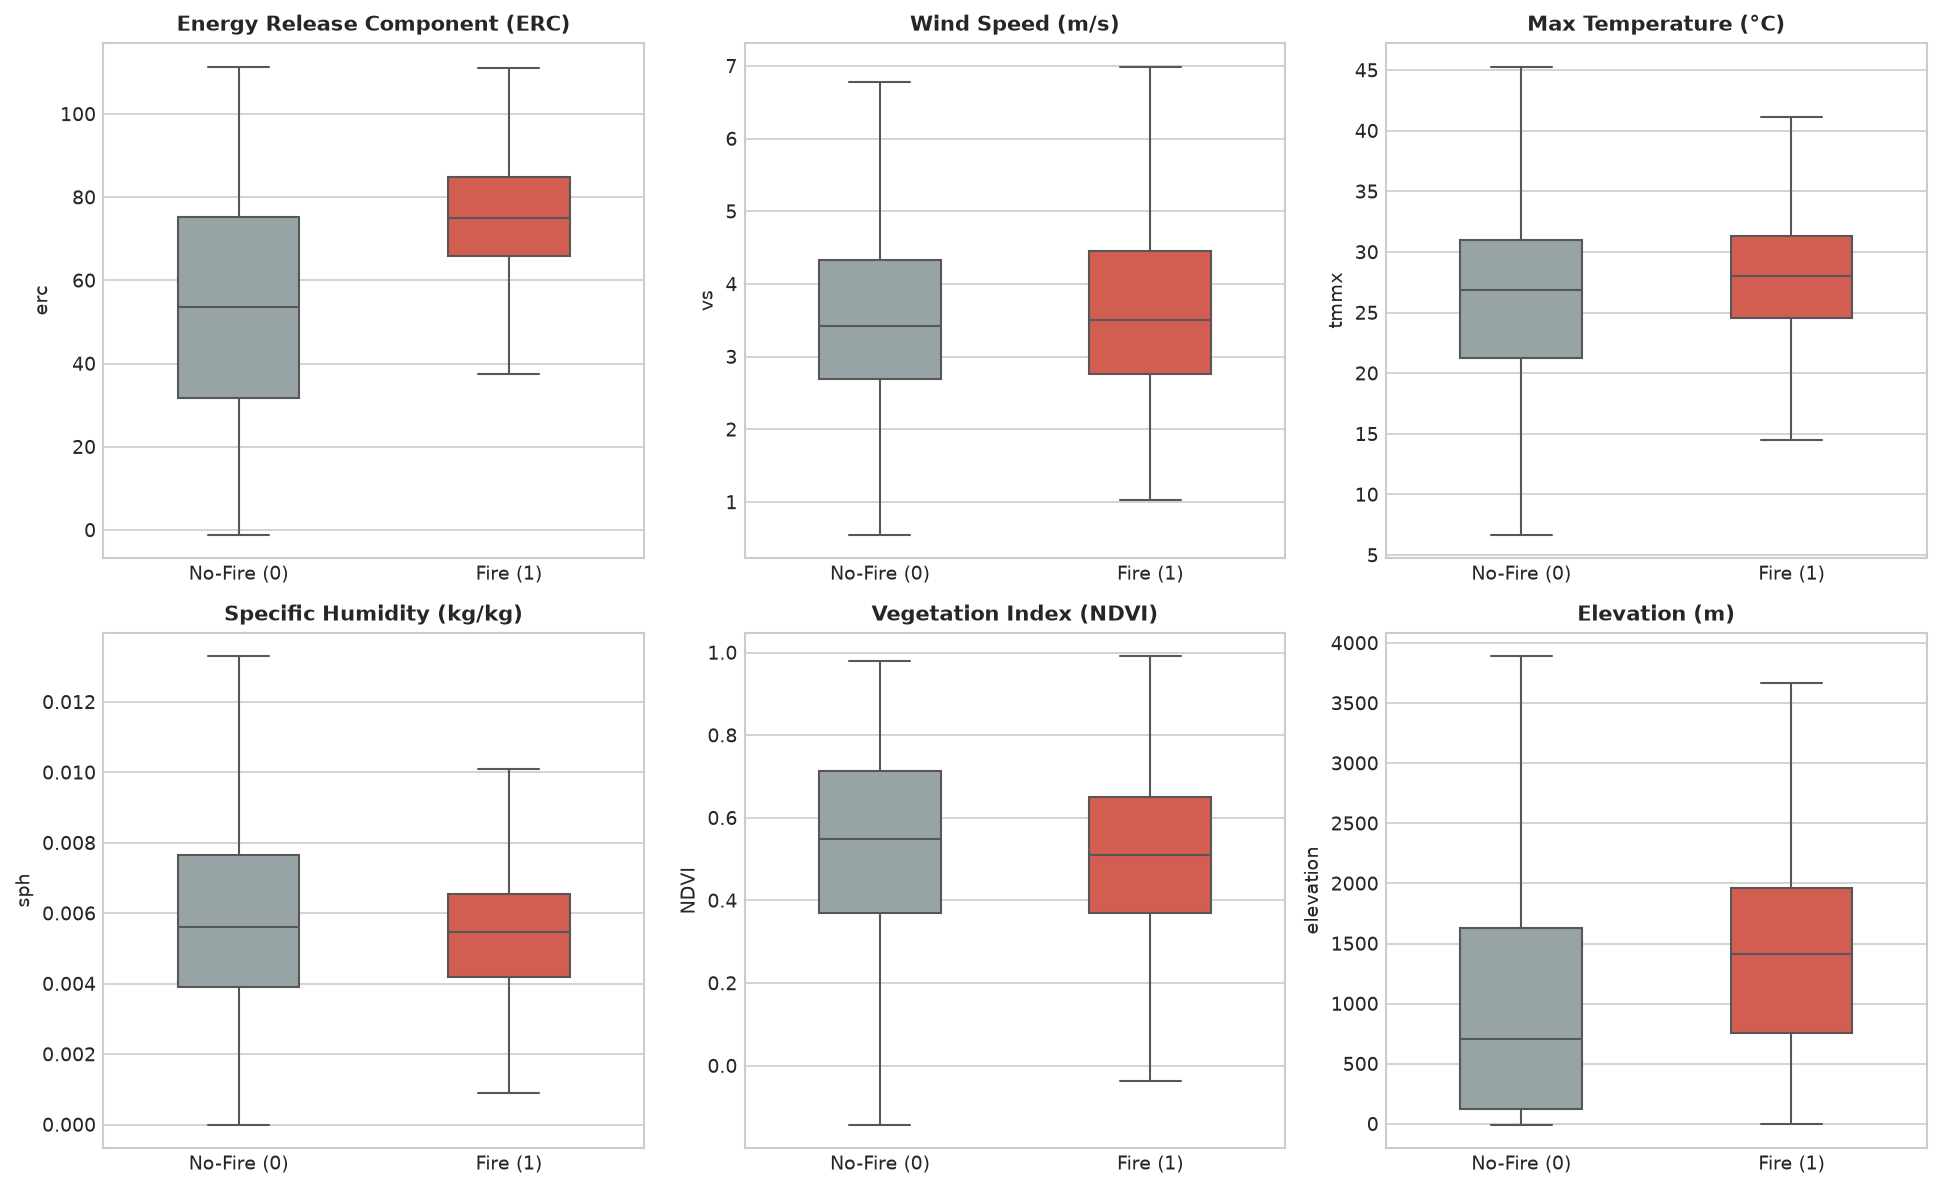
\includegraphics[width=\columnwidth]{figures/eda_fire_vs_nofire_features.png}
\caption{Raw channel distributions for next-day fire vs.\ no-fire pixels (balanced 50k/50k training
sample, outliers hidden).}
\label{fig:fire_vs_nofire}
\end{figure}

\subsection{From EDA to features}
Three findings shaped the pipeline. (i) A pixel's own weather says little about whether it burns,
while burning depends strongly on nearby fire, so most engineered features describe the fire
neighbourhood (Table~\ref{tab:features}). (ii) Measuring each next-day fire pixel's distance to the
nearest day-$t$ fire shows that 40.4\% lie more than 5\,km away and 26.1\% more than 10\,km away;
we therefore added an upwind fire feature at 8\,km (\texttt{upwind\_fire\_k8}), which ranks 5th of
35 features by gain in the tuned XGBoost. (iii) Wind direction is circular, so out-of-range values
are wrapped rather than clipped. We did not clip negative NDVI, because water and snow are genuine,
informative non-fuel.

\subsection{Feature-group ablation}
To measure what each feature group contributes, we retrain the tuned LightGBM with identical
hyperparameters while removing one group at a time, plus a run with the fire-neighbourhood group
only (Table~\ref{tab:ablation}, Fig.~\ref{fig:ablation}). Each run chooses its F1 threshold on eval
and is scored on test. Removing the fire-neighbourhood features collapses PR AUC from 0.248 to 0.048,
mirroring Huot et al., where removing the previous fire mask cuts PR AUC from 28.4\% to 6.8\%.
Among the environmental groups, vegetation matters most ($-0.009$), again in line with Huot et al.,
who found vegetation the most useful variable alongside the fire mask. Removing weather costs only
0.001, and removing terrain or population changes PR AUC by $+0.003$ and $+0.002$; differences this
small are within run-to-run noise and suggest these groups overlap with the remaining features.
The fire-neighbourhood features alone reach 0.218, so the environmental variables add 0.031
(14\%) on top of fire location. Because the upwind and alignment features use wind direction,
the ``no weather'' run still sees some wind information.

\begin{table}[t]
\centering
\caption{Feature-group ablation (LightGBM, test split, F1 at eval-chosen threshold).}
\label{tab:ablation}
\begin{tabular}{lrrrr}
\hline
Run & \#feat. & PR AUC & $\Delta$ & F1 \\
\hline
All features & 35 & 0.248 & -- & 0.331 \\
No weather & 21 & 0.248 & $-0.001$ & 0.334 \\
No vegetation & 31 & 0.240 & $-0.009$ & 0.333 \\
No terrain & 30 & 0.251 & $+0.003$ & 0.340 \\
No fire neighbourhood & 25 & 0.048 & $-0.200$ & 0.093 \\
No human & 33 & 0.251 & $+0.002$ & 0.336 \\
Fire neighbourhood only & 10 & 0.218 & $-0.031$ & 0.334 \\
\hline
\end{tabular}
\end{table}

\begin{figure}[t]
\centering
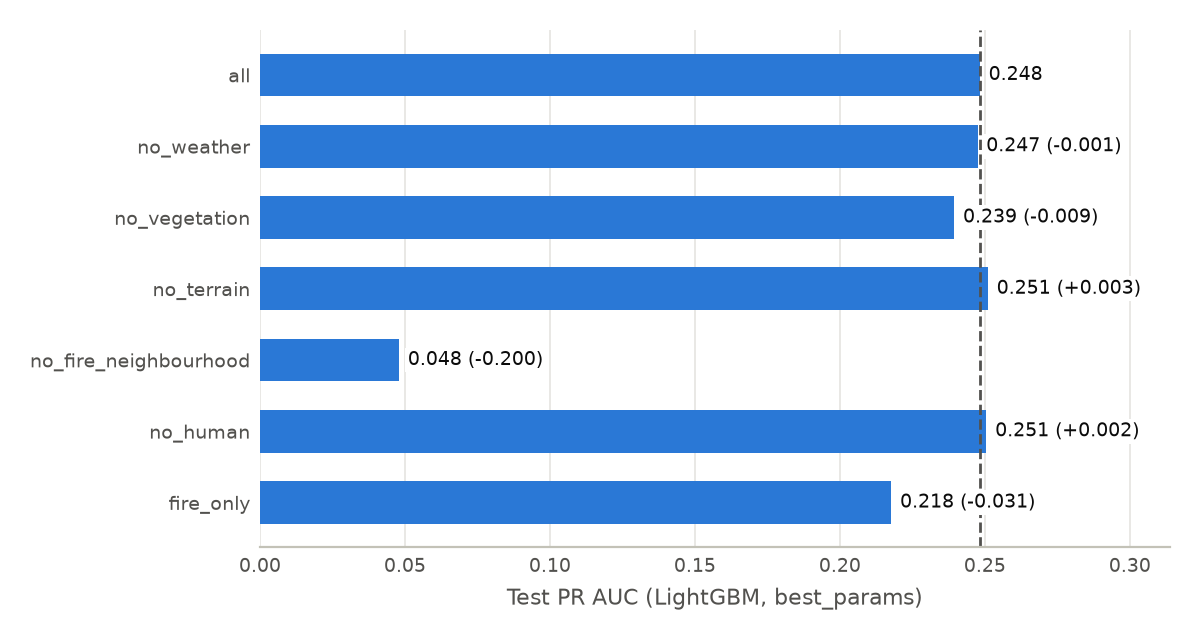
\includegraphics[width=\columnwidth]{figures/ablation_pr_auc.png}
\caption{Test PR AUC per ablation run; the dashed line marks the model with all features.}
\label{fig:ablation}
\end{figure}

% Methodology and Feature Engineering

\section{Methodology}

\subsection{Problem formulation}
Each sample of the Next Day Wildfire Spread dataset~\cite{huot2022} is a $64\times64$ patch at
1\,km resolution with 12 input channels observed on day $t$ (11 environmental channels plus the
active fire mask \texttt{PrevFireMask}) and a target fire mask \texttt{FireMask} on day $t+1$.
We treat the task as per-pixel binary classification: for every pixel, predict the probability
that it is burning on day $t+1$ using only information available on day $t$.
Pixels with label $-1$ (unknown, e.g.\ cloud cover) are excluded from training and from every metric.

\subsection{Data splits}
We use the official train/eval/test split released with the dataset
(14\,979 / 1\,877 / 1\,689 patches). Huot et al.\ assign every calendar week between 2012 and 2020
at random to train, eval or test in an 8:1:1 ratio and leave a one-day buffer between weeks, so
the splits are separated in time and a fire's day-$t$/day-$t{+}1$ pair never straddles two splits.
All features are computed inside a single patch, so no feature uses pixels from another sample. The
week-based split separates samples in time, but it does not guarantee spatial or fire-event
independence: a long-lived fire can appear in weeks assigned to different splits. We have not checked
for such overlap.
The eval split is used only for early stopping and hyperparameter selection;
the test split is scored once per final model.

\subsection{Preprocessing}
The TFRecords are parsed directly from the protobuf wire format (no TensorFlow dependency) into
arrays of shape $(N,12,64,64)$. The raw export contains physically impossible values,
so before feature construction each affected channel is clipped to fixed physical bounds
(Table~\ref{tab:clip}). Wind direction is circular, so instead of clipping it is wrapped
($\theta \bmod 360$; 0.23\% of train pixels lie outside $[0, 360)$).
The dataset does not state the patch orientation, so we verified it from the data: the arrays are
stored south-up (the row index grows northward). Steep slopes facing the last row are clearly
greener than those facing the first row (mean NDVI 0.596 vs.\ 0.555, while east- and west-facing
slopes differ by only 0.008), as expected for pole-facing slopes in the Northern Hemisphere, and only
this orientation makes next-day fire more frequent downwind than upwind in every wind-speed band
(from 1.1$\times$ in calm wind to 3.1$\times$ at 8\,m/s or more, 5\,km from the fire; Results section). All
direction-dependent features (upwind fire, wind alignment, aspect) use this orientation. The bounds are constants, not statistics fitted on the data, so clipping
introduces no leakage. No normalisation is applied for the tree models, which are invariant to
monotone rescaling of individual features.

\begin{table}[t]
\centering
\caption{Physical clipping of raw channels (train split shares of affected pixels).}
\label{tab:clip}
\begin{tabular}{lll}
\hline
Channel & Bounds & Affected pixels \\
\hline
\texttt{vs} (wind speed) & $\geq 0$ m/s & $<0.01$\% \\
\texttt{tmmn}, \texttt{tmmx} & $[253.15, 330]$ K & 0.36\% \\
\texttt{sph} & $\geq 0$ & $<0.01$\% \\
\texttt{pr} & $\geq 0$ mm & 9.78\% \\
\texttt{erc} & $\geq 0$ & 0.03\% \\
\hline
\end{tabular}
\end{table}

\subsection{Pixel tables and class imbalance}
Fire pixels are rare: on the training split only 1.1\% of labelled pixels burn on day $t+1$
(a 90:1 imbalance). Each patch is flattened into one row per pixel. For the training table we
keep every fire pixel and an independent random sample of non-fire pixels with probability chosen
to give a 5:1 non-fire to fire ratio (fixed seed), giving 3.95\,M rows.
Uniform negative subsampling shifts the predicted base rate but not the ranking of pixels,
so ranking metrics on the untouched eval and test splits remain valid.
The remaining imbalance is handled by class weighting computed from the training table only:
\texttt{scale\_pos\_weight} $= N_{\text{neg}}/N_{\text{pos}} = 5$.
Eval (7.69\,M pixels) and test (6.92\,M pixels) keep every pixel in patch order, so predictions
reshape directly into $64\times64$ probability maps.

\subsection{Models and tuning}
We train XGBoost~\cite{chen2016} and LightGBM~\cite{ke2017} on all 35 features (12 raw plus 23
engineered). For each family we run a random search of 20 configurations over the space in
Table~\ref{tab:space}. Every configuration grows up to 1\,000 trees with early stopping
(patience 50) on a fixed random sample of 1\,M labelled eval pixels, and is then scored by
PR AUC on the full eval split. The best configuration per family is evaluated once on test.

\begin{table}[t]
\centering
\caption{Random search spaces (20 configurations each).}
\label{tab:space}
\begin{tabular}{lll}
\hline
Model & Hyperparameter & Range \\
\hline
XGBoost & \texttt{max\_depth} & \{4, 6, 8, 10\} \\
 & \texttt{min\_child\_weight} & \{1, 5, 20, 100\} \\
 & \texttt{gamma} & \{0, 0.1, 1\} \\
LightGBM & \texttt{num\_leaves} & \{15, 31, 63, 127, 255\} \\
 & \texttt{min\_child\_samples} & \{20, 100, 500, 2000\} \\
 & \texttt{min\_split\_gain} & \{0, 0.1, 1\} \\
Both & \texttt{learning\_rate} & log-uniform $[0.02, 0.3]$ \\
 & \texttt{subsample} & uniform $[0.6, 1]$ \\
 & \texttt{colsample\_bytree} & uniform $[0.5, 1]$ \\
 & \texttt{reg\_lambda} & log-uniform $[0.1, 10]$ \\
\hline
\end{tabular}
\end{table}

Eval PR AUC varied little across configurations (XGBoost 0.196--0.207, LightGBM 0.189--0.203),
so the results are not sensitive to the exact hyperparameters. The selected XGBoost uses depth 6,
learning rate 0.026 and 216 trees; the selected LightGBM uses 15 leaves, at least 500 samples
per leaf, learning rate 0.058 and 294 trees. Full configurations are in
\texttt{reports/best\_params.json}.

\subsection{Evaluation}
Accuracy is uninformative at 1\% prevalence, so every model is scored with the same function on
the same pixels: PR AUC (average precision), ROC AUC, and recall at 1\% and 5\% false positive
rate, which need no decision threshold. Precision, recall and F1 are reported at the threshold
that maximises F1 on the eval split, applied unchanged to test; choosing it on test would
overstate F1. The test-optimal F1 is kept only as an upper bound.

\section{Feature Engineering}
Raw channels describe each pixel in isolation, but fire spread depends on where the fire is,
which way the wind blows relative to it, how dry the air and fuel are, and the local terrain.
We engineer 23 features in five groups (Table~\ref{tab:features}); the groups are reused for the
ablation study. Unless stated, local statistics use a $k\times k$ window with replicated edges,
\texttt{PrevFireMask} $=-1$ is treated as no fire, and wind direction $\theta$ is the direction
the wind blows \emph{from} (degrees clockwise from north).

\begin{table*}[t]
\centering
\caption{Engineered features. AUC: univariate ROC AUC on the eval split, $\max(a, 1-a)$,
sign gives direction of association. Raw channel shown for comparison.}
\label{tab:features}
\begin{tabular}{llll}
\hline
Group & Feature & Definition & AUC \\
\hline
Fire & \texttt{PrevFireMask} (raw) & fire on day $t$ & 0.593 (+) \\
 & \texttt{prev\_fire\_n3/n5/n9} & mean of fire indicator in $3/5/9$ window & 0.668 / 0.717 / 0.772 (+) \\
 & \texttt{patch\_fire\_frac} & fraction of patch burning & 0.759 (+) \\
 & \texttt{dist\_to\_fire} & Euclidean distance to nearest fire (px $\approx$ km), $64\sqrt2$ if none & 0.866 ($-$) \\
 & \texttt{upwind\_fire\_k2/k4/k8} & \texttt{prev\_fire\_n3} at the pixel $2/4/8$ px upwind & 0.649 / 0.615 / 0.586 (+) \\
 & \texttt{fire\_wind\_alignment} & $\cos$(upwind direction, direction to nearest fire) & 0.501 \\
\hline
Weather & \texttt{sph} (raw) & specific humidity & 0.565 ($-$) \\
 & \texttt{wind\_u}, \texttt{wind\_v} & $-v_s\sin\theta$, $-v_s\cos\theta$ & 0.522 / 0.518 \\
 & \texttt{temp\_range} & \texttt{tmmx} $-$ \texttt{tmmn} & 0.602 (+) \\
 & \texttt{vpd} & $e_s(T_{\max}) - e$ & 0.685 (+) \\
 & \texttt{min\_rel\_humidity} & $e / e_s(T_{\max})$ & 0.705 ($-$) \\
 & \texttt{erc\_x\_wind} & \texttt{erc} $\times v_s$ & 0.679 (+) \\
\hline
Vegetation & \texttt{NDVI} (raw) & NDVI $\times10^4$ & 0.605 ($-$) \\
 & \texttt{ndvi\_n5\_mean/std} & local mean / std of NDVI, $5\times5$ & 0.610 ($-$) / 0.513 \\
 & \texttt{ndvi\_anomaly} & NDVI $-$ local mean & 0.508 \\
\hline
Terrain & \texttt{elevation} (raw) & SRTM elevation, m & 0.626 (+) \\
 & \texttt{slope} & $\arctan\lVert\nabla z\rVert$, degrees & 0.677 (+) \\
 & \texttt{aspect\_sin/cos} & downslope direction & 0.508 \\
 & \texttt{elev\_rel} & $z - $ mean of $z$ in $9\times9$ & 0.527 (+) \\
\hline
Human & \texttt{population} (raw) & people / km$^2$ & 0.601 ($-$) \\
 & \texttt{pop\_n9} & mean population in $9\times9$ & 0.628 ($-$) \\
\hline
\end{tabular}
\end{table*}

\textbf{Fire neighbourhood.} Spread happens at the fire front, so we measure burning density
around each pixel at three scales, the distance to the nearest burning pixel, and the fraction of
the patch already burning. Three wind-aware features look for fire $k \in \{2,4,8\}$ pixels upwind (8 because 40\% of
next-day fire pixels lie more than 5\,km from day-$t$ fire, per our EDA), and an
alignment score is the cosine between the upwind direction and the direction to the nearest fire
($+1$ when the wind pushes the nearest fire toward the pixel).

\textbf{Weather.} Wind direction is circular, so it is replaced by $u$/$v$ components.
Specific humidity is converted to vapour pressure $e = qp/(0.622+0.378q)$, with surface pressure
$p$ from elevation (FAO-56). Saturation vapour pressure at the daily maximum temperature,
$e_s = 0.6108\exp\!\big(17.27T/(T+237.3)\big)$ kPa, gives the vapour pressure deficit
$e_s - e$ and minimum relative humidity $e/e_s$, both direct measures of atmospheric drying.
We also add diurnal temperature range and the interaction \texttt{erc}$\times$wind speed.

\textbf{Vegetation, terrain, human.} NDVI (stored $\times10^4$) is summarised by its local mean,
standard deviation and anomaly. Terrain adds slope and aspect from the elevation gradient and
elevation relative to the $9\times9$ neighbourhood (ridges vs.\ valleys). Population is
smoothed over $9\times9$ pixels as a proxy for settlement proximity and suppression effort.


Engineered features consistently carry more signal than the raw channels they are built from:
\texttt{dist\_to\_fire} reaches a univariate AUC of 0.866 against 0.593 for the raw fire mask,
and \texttt{min\_rel\_humidity} 0.705 against 0.565 for specific humidity.
\texttt{fire\_wind\_alignment} has no marginal signal (0.501) because it is only meaningful close
to an active fire, and gain importance in the tuned XGBoost shows the model barely uses it
(23rd of 35 features, 0.5\% of total gain). The fire-neighbourhood group dominates instead:
\texttt{dist\_to\_fire} (32\%), \texttt{prev\_fire\_n9} (23\%) and \texttt{prev\_fire\_n5} (13\%).
The three upwind features rank 4th, 5th and 7th and together hold 13.5\% of gain;
\texttt{upwind\_fire\_k8}, added after the EDA showed long-range spread, ranks 5th (3.9\%).
With the patch orientation corrected, their combined share rose from 9.4\% to 13.5\%,
so the model uses wind direction more once upwind is computed on the correct side.
The raw \texttt{PrevFireMask} ranks only 32nd because the engineered neighbourhood features already
contain its information.

% Results
% Every number comes from reports/results.csv, reports/results_table.md, notebooks/02_evaluation.ipynb
% or reports/checks.

\section{Results}

All models are scored on the same 6\,727\,699 labelled test pixels (1\,689 patches); 1.25\% of them burn on
day $t+1$, about one pixel in 80. Precision, recall and F1 use the threshold that maximises F1 on the eval split;
PR AUC, ROC AUC and recall at a fixed false positive rate (FPR) need no threshold.

\subsection{Overall performance}

\begin{table*}[t]
\centering
\caption{Test results. Precision (P), recall (R) and F1 at the threshold chosen on the eval split. Bold: best per
column. PR AUC reported by Huot et al.~\cite{huot2022} for their models is in Table~\ref{tab:relwork}.}
\label{tab:results}
\begin{tabular}{lccccccc}
\hline
Model & PR AUC & ROC AUC & P & R & F1 & R @ 1\% FPR & R @ 5\% FPR \\
\hline
Persistence & 0.106 & 0.633 & 0.357 & 0.273 & 0.309 & 0.273 & 0.273 \\
Logistic regression (raw) & 0.146 & 0.798 & \textbf{0.378} & 0.266 & 0.312 & 0.281 & 0.319 \\
Random forest (raw) & 0.157 & 0.816 & 0.371 & 0.270 & 0.312 & 0.279 & 0.362 \\
XGBoost (raw) & 0.145 & 0.795 & 0.337 & 0.257 & 0.292 & 0.267 & 0.375 \\
XGBoost (tuned, 35 features) & \textbf{0.257} & \textbf{0.906} & 0.242 & \textbf{0.526} & \textbf{0.332} & \textbf{0.388} & \textbf{0.675} \\
LightGBM (tuned, 35 features) & 0.248 & 0.903 & 0.242 & 0.520 & 0.331 & 0.384 & 0.671 \\
\hline
\end{tabular}
\end{table*}

\begin{figure*}[!t]
\centering
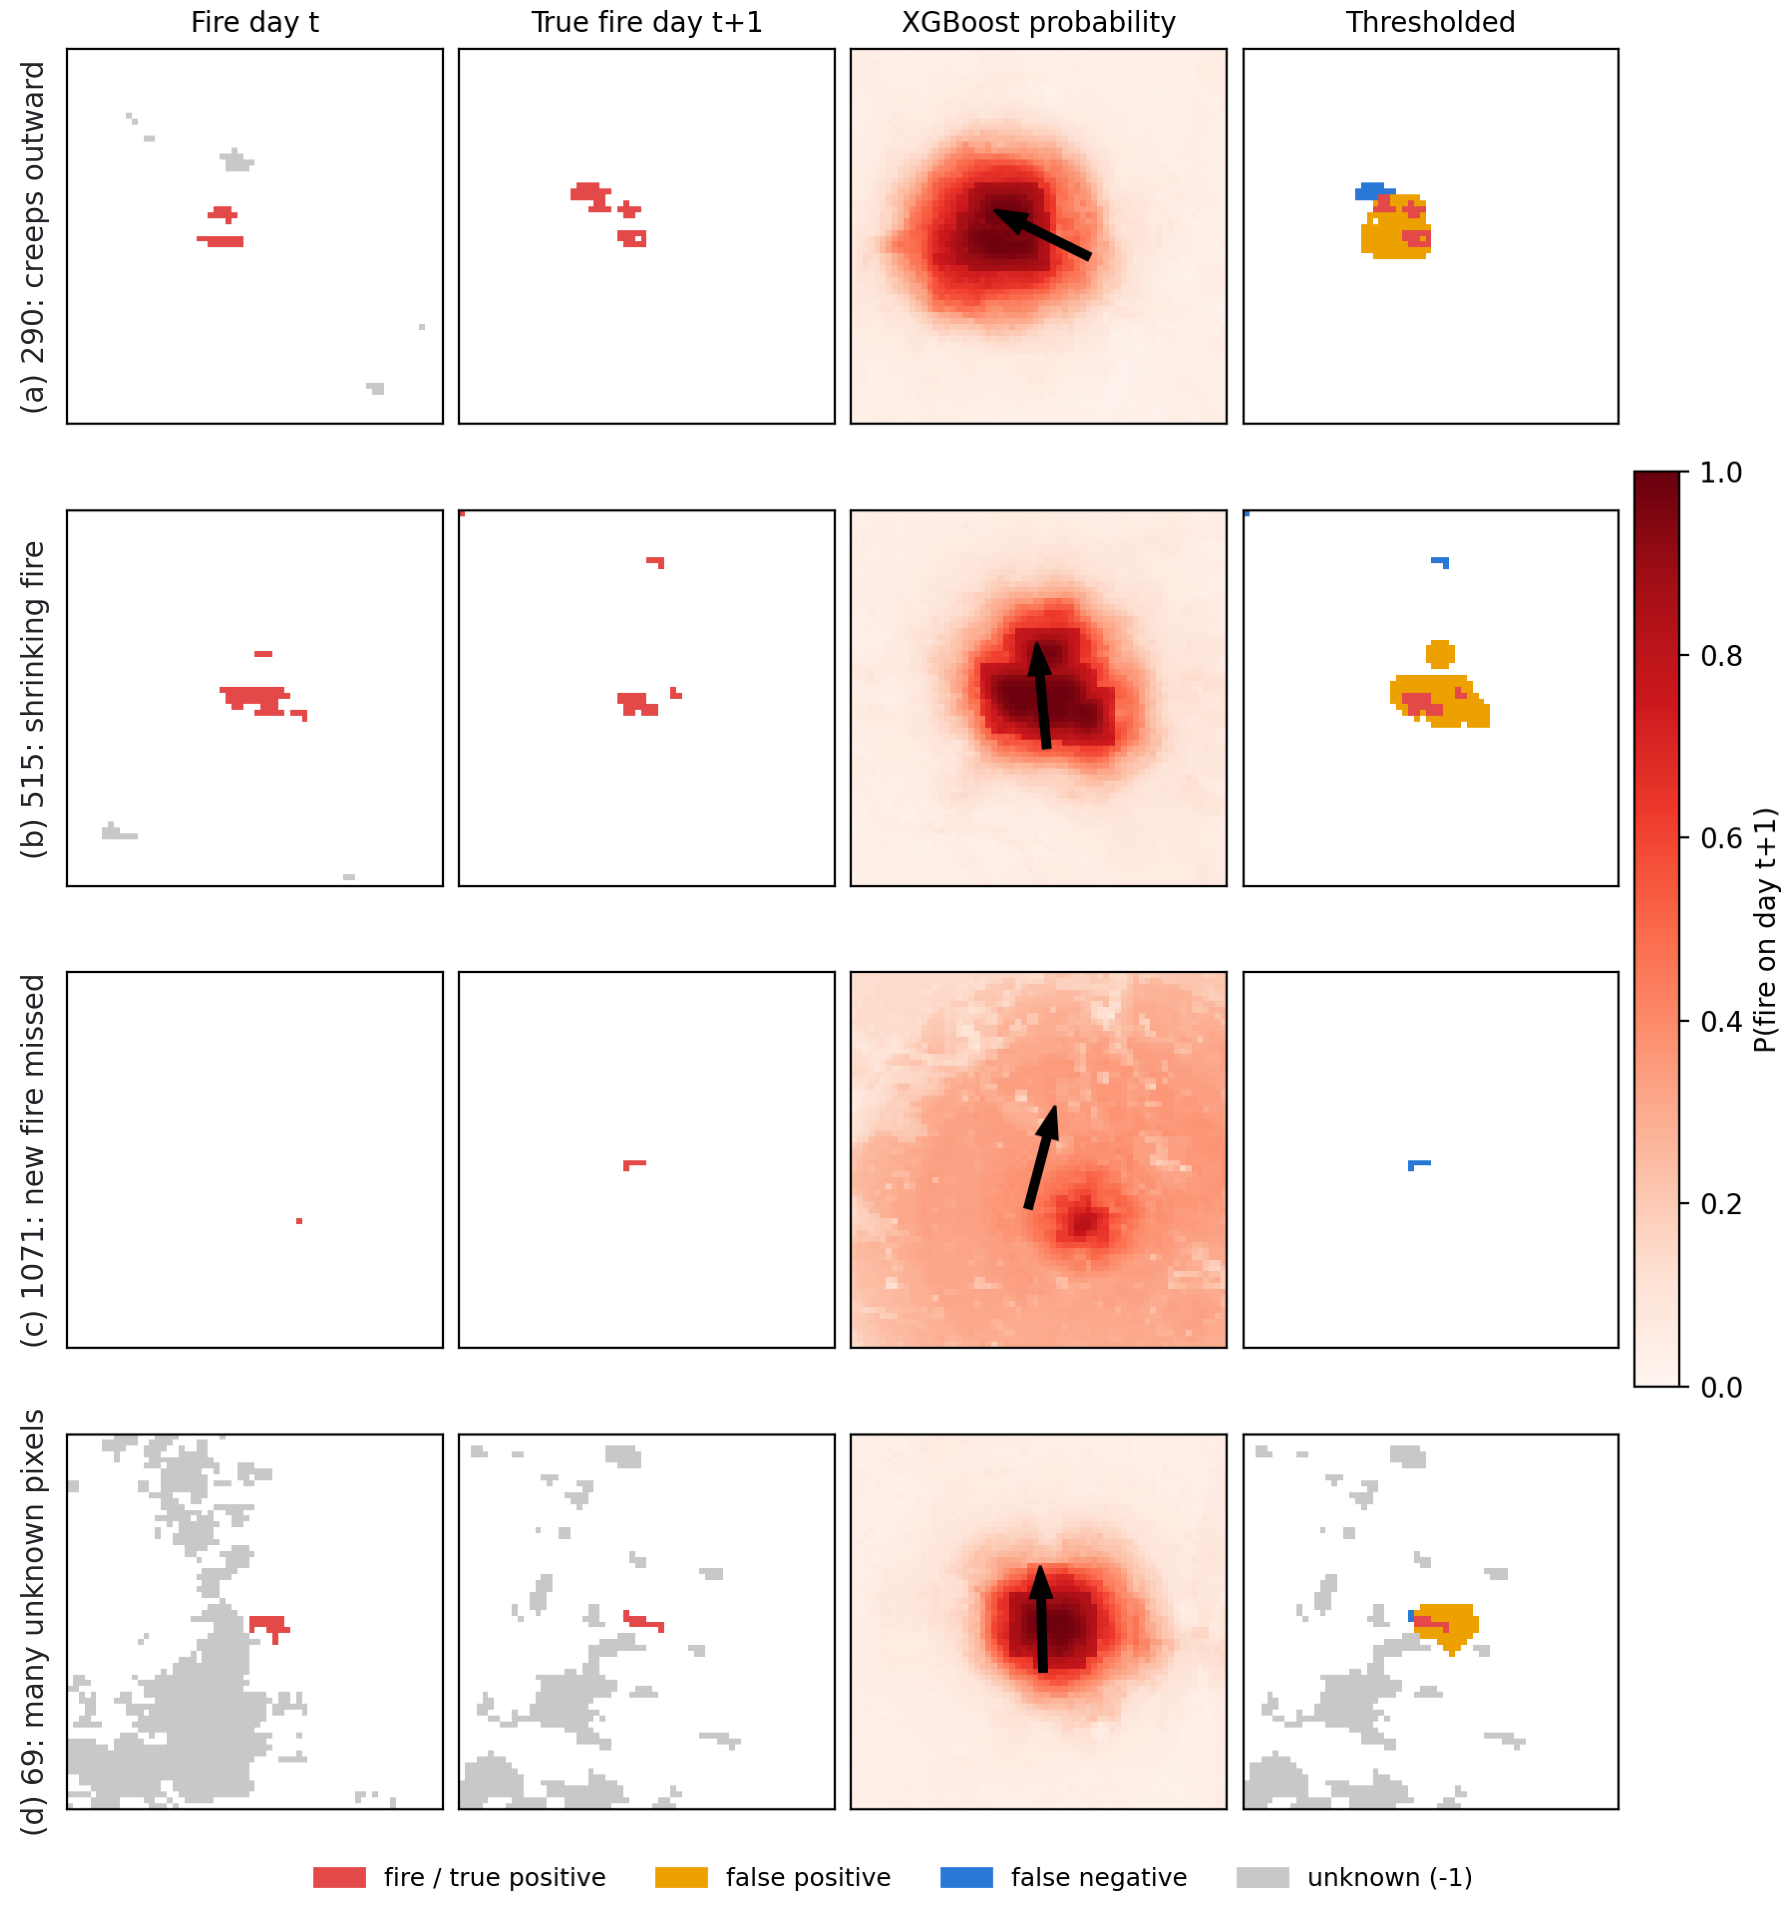
\includegraphics[width=0.72\textwidth]{figures/eval_prob_maps_selected.png}
\caption{Tuned XGBoost on four test patches that show its typical behaviour (all ten random patches are in
Fig.~\ref{fig:maps_all}). Columns: fire on day $t$, true fire on day $t+1$, predicted probability (arrow: direction the
wind blows to), and prediction at the eval threshold. Drawn from the rebuilt model (Appendix~\ref{app:checks}).}
\label{fig:maps}
\end{figure*}

The tuned XGBoost is the best model on every threshold-free metric (Table~\ref{tab:results}): PR AUC 0.257 against
0.145--0.157 for the raw-channel models and 0.106 for persistence. LightGBM is close behind (0.248), so the features
matter far more than the boosting library; the ablation (Table~\ref{tab:ablation}) traces the gain to the
fire-neighbourhood group. At the eval threshold the tuned models find 52--53\% of next-day fire at 24\% precision,
about twice the recall of the baselines (26--27\%), and reach the best F1 (0.332); a threshold tuned on test would give
only 0.358, so the eval threshold transfers well. Our persistence (0.106) is close to the paper's (0.115); the tuned
XGBoost is above their neighbour-feature random forest (0.225) but below their CNN (0.284). Both values lie inside our
95\% bootstrap interval over fire events (0.188-0.325, Appendix~\ref{app:checks}), so neither difference is significant
on test-sampling grounds. The same check shows that the gap to LightGBM is small but consistent (0.007, higher in 99\%
of paired resamples), and the gain over the raw-channel models clear (0.10, interval 0.09-0.12).

\begin{figure}[t]
\centering
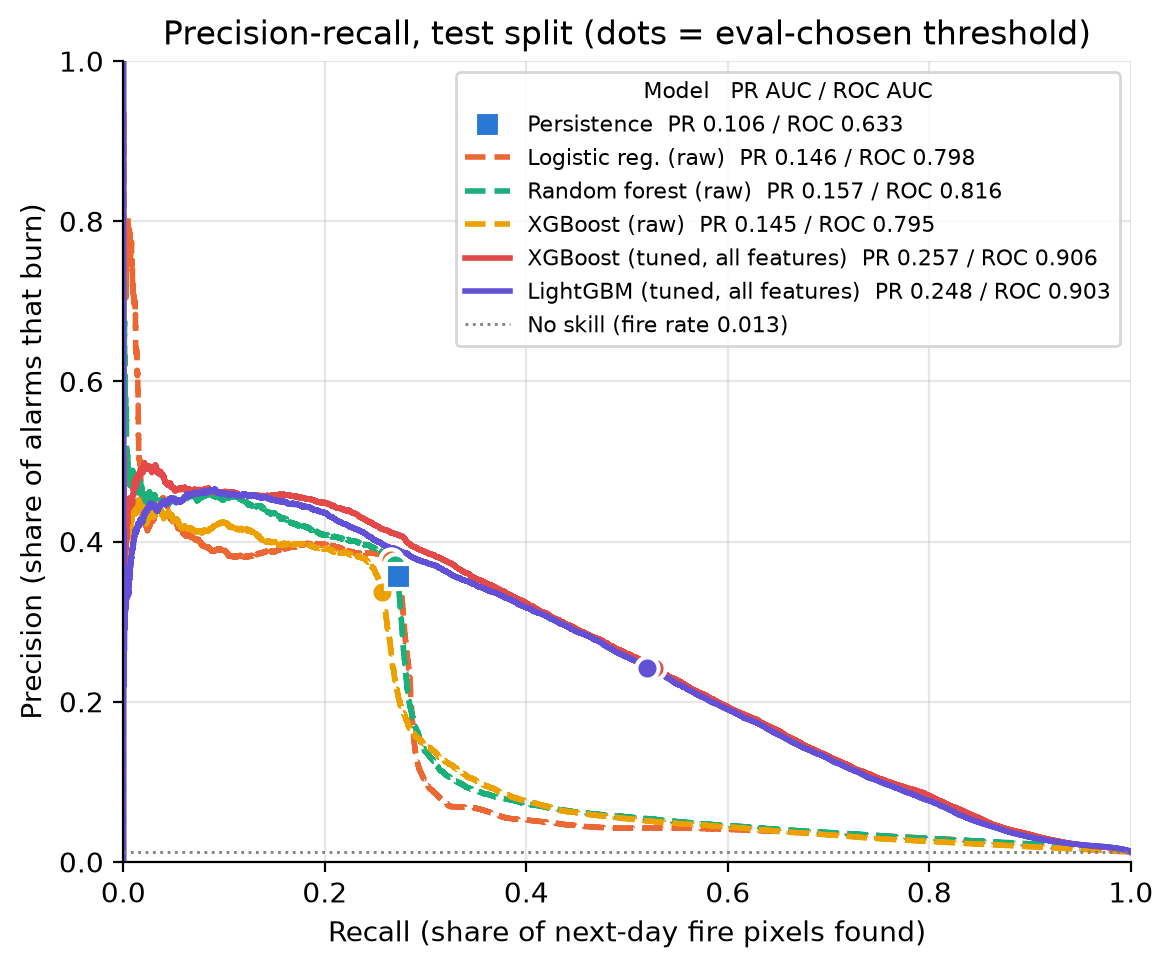
\includegraphics[width=\columnwidth]{figures/eval_pr_curves.png}
\caption{Precision--recall curves on the test split. Dots: operating point at the eval-chosen threshold.
Persistence outputs only 0 or 1, so it is a single point.}
\label{fig:pr}
\end{figure}

The tuned models stay above every baseline along the whole PR curve (Fig.~\ref{fig:pr}). The raw-channel models rank
already-burning pixels first and have little signal for new fire, so their operating points sit on top of persistence.
ROC AUC is 0.795--0.906 for every learned model while PR AUC stays at or below 0.257; Section~\ref{sec:theory_pr}
explains why PR AUC is the more informative metric at this prevalence.

\subsection{Probability maps}

The predicted probability is a smooth halo around the day-$t$ fire (Fig.~\ref{fig:maps}), following its shape and
stretched slightly toward where the wind blows (Fig.~\ref{fig:maps}d; patch 33 in Fig.~\ref{fig:maps_all}). After
thresholding, the prediction is roughly the day-$t$ fire grown by a few kilometres. It catches fire that stays or creeps
outward (Fig.~\ref{fig:maps}a; also patches 856 and 1432), paints a false-positive ring around small fires that shrink
(Fig.~\ref{fig:maps}b, patch 515: 48 to 29 burning pixels, 114 false positives), and misses fire that appears away from
the day-$t$ fire (Fig.~\ref{fig:maps}c): in patches 120, 443, 1071 and 1369 not one next-day fire pixel is found.
Unknown pixels (grey) are left out of every metric. The raw scores are shifted by the 5:1 subsampled table and the class
weighting, which is why the eval threshold is as high as 0.915; undoing that shift in closed form gives probabilities
close to the observed fire rate (Section~\ref{sec:theory_imb}). Only the ranking and the threshold affect the metrics.

\subsection{Interpretability and physical plausibility}

\begin{figure}[t]
\centering
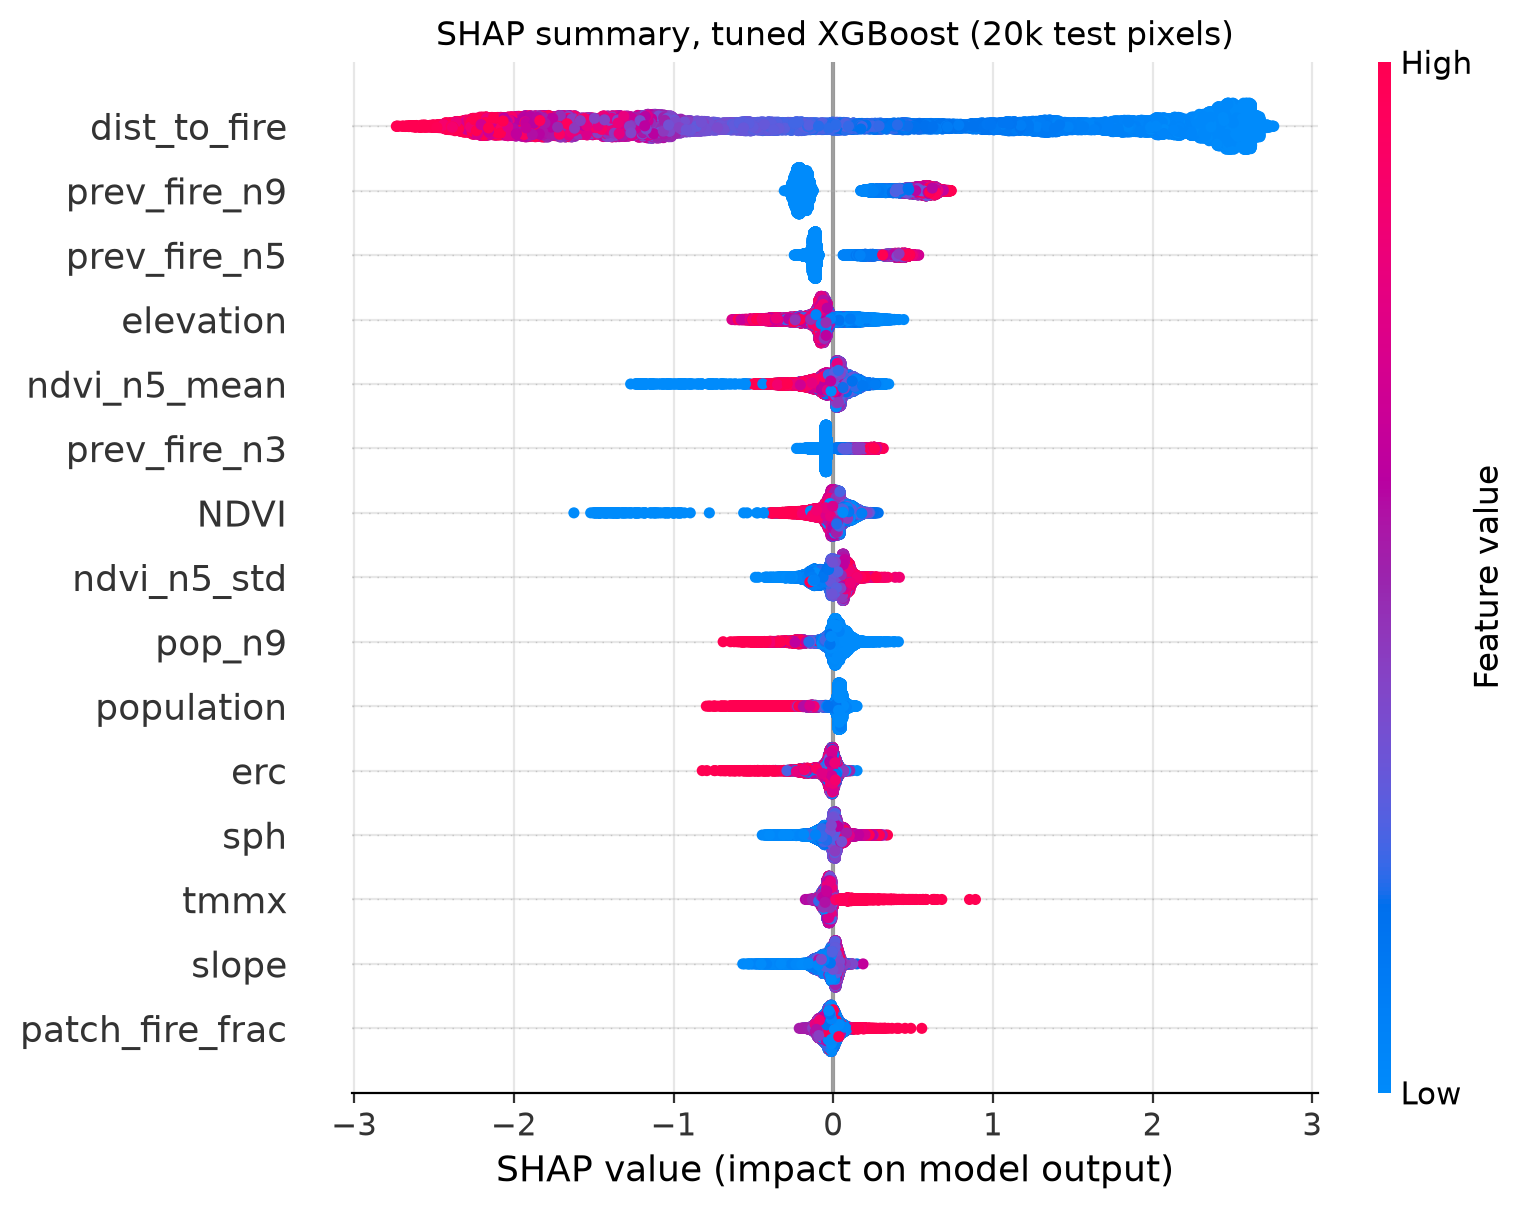
\includegraphics[width=\columnwidth]{figures/eval_shap_summary.png}
\caption{SHAP values of the tuned XGBoost on 20\,000 test pixels (10\,000 fire, 10\,000 no fire). Positive values push
the prediction toward fire; colour shows the feature value.}
\label{fig:shap}
\end{figure}

SHAP values~\cite{lundberg2017}, computed with TreeSHAP~\cite{lundberg2020}, of the refitted model (identical predictions, Fig.~\ref{fig:shap}) confirm the gain ranking in the Feature
Engineering section: the fire-neighbourhood group contributes 2.29 log-odds on average, against 0.40 for weather, 0.22
for vegetation, 0.20 for terrain and 0.13 for human features. Most effects have the expected sign (Spearman $\rho$
between feature value and SHAP value):
pixels closer to fire and with more fire nearby get higher risk (\texttt{dist\_to\_fire} $-0.97$,
\texttt{prev\_fire\_n3} $+0.75$); drier air raises it
(\texttt{vpd} $+0.72$, \texttt{min\_rel\_humidity} $-0.64$); and so do stronger wind (\texttt{vs} $+0.72$) and fire
upwind (\texttt{upwind\_fire\_k2/k4/k8} $+0.69/+0.61/+0.49$, \texttt{fire\_wind\_alignment} $+0.91$). NDVI is
mixed: bare ground and water (lowest NDVI, no fuel) get the most negative SHAP values, while over the main range greener,
moister vegetation lowers risk ($\rho=-0.82$). One sign is not physical: high ERC (dry fuel) lowers the prediction ($\rho=-0.13$ overall, with the strongest negative SHAP values
at the highest ERC). ERC is a coarse regional value, almost constant over a patch, so the model most likely uses it as a
proxy for where and when a fire is, not as a cause.

\begin{figure}[t]
\centering
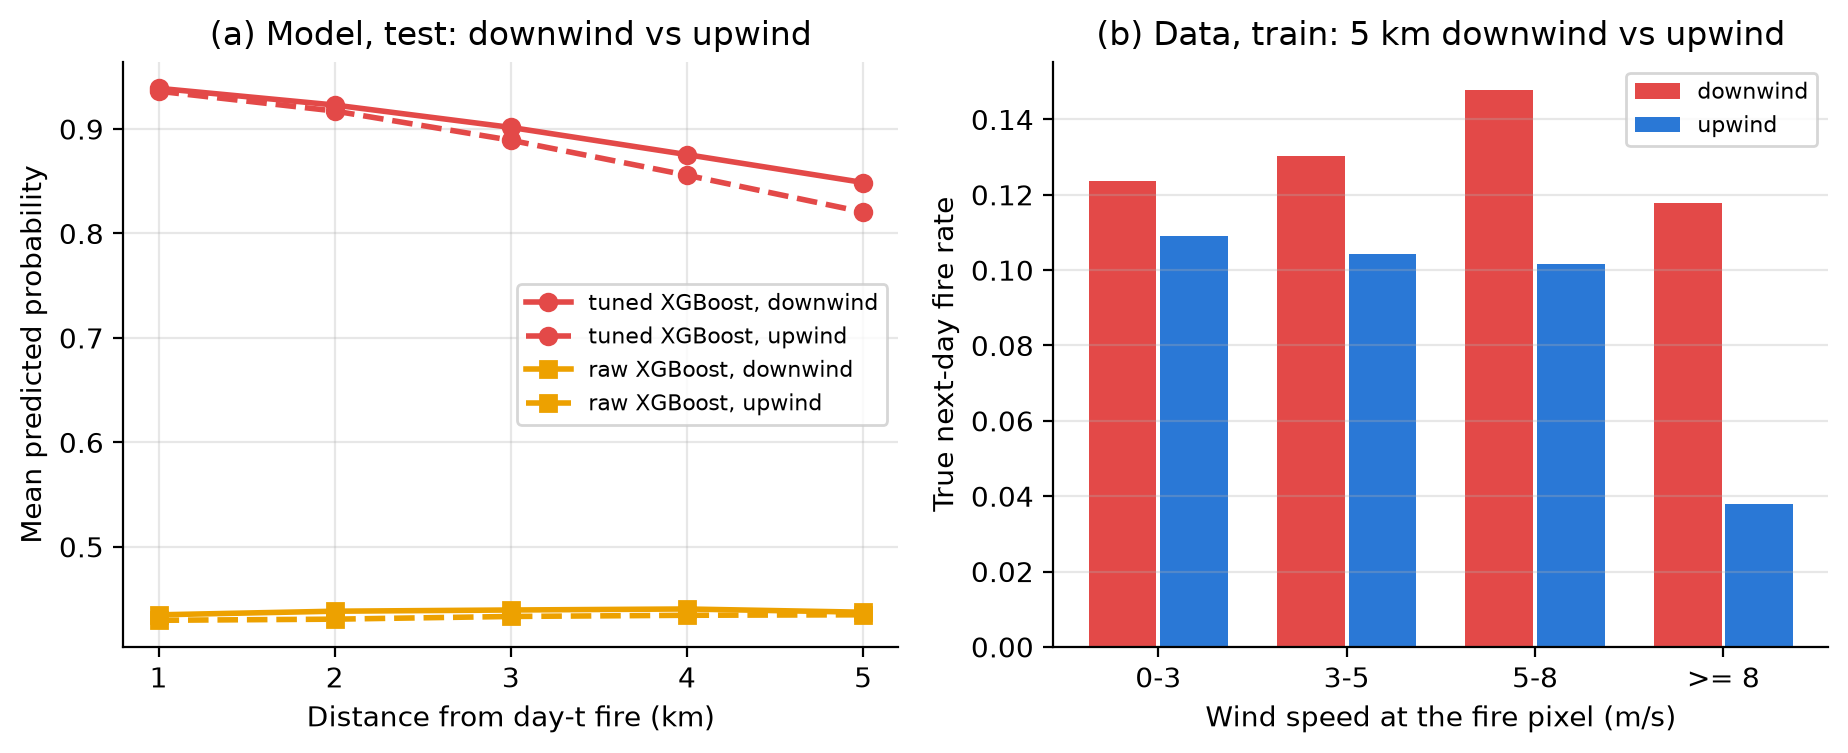
\includegraphics[width=\columnwidth]{figures/eval_downwind_check.png}
\caption{Downwind check. (a) Mean predicted probability 1--5\,km downwind (solid) and upwind (dashed) of day-$t$ fire,
test split. (b) True next-day fire rate 5\,km downwind and upwind of day-$t$ fire by wind speed, train split.}
\label{fig:wind}
\end{figure}

To test whether the model pushes risk downwind, we step 1--5 pixels downwind and upwind from every day-$t$ fire pixel
and compare predictions in pixels not yet burning (Fig.~\ref{fig:wind}a). The tuned model's downwind probability is
higher at every distance, with the gap growing from 0.003 at 1\,km to 0.029 at 5\,km. The training data agrees
(Fig.~\ref{fig:wind}b): 5\,km from the fire, the downwind-to-upwind ratio of next-day fire grows with wind speed, from
1.135 in calm wind (0--3\,m/s) to 3.100 at 8\,m/s or more. Our first version of this check assumed north-up patches and
found the opposite in strong wind, which revealed that the arrays are stored south-up. On test the excess holds only in
calm wind (1.081, against 0.782 and 0.444 at 3--8\,m/s), but these ratios rest on a few large fires
(Section~\ref{sec:events}), so the train split is the more reliable estimate.

\subsection{Error analysis}

\begin{figure}[t]
\centering
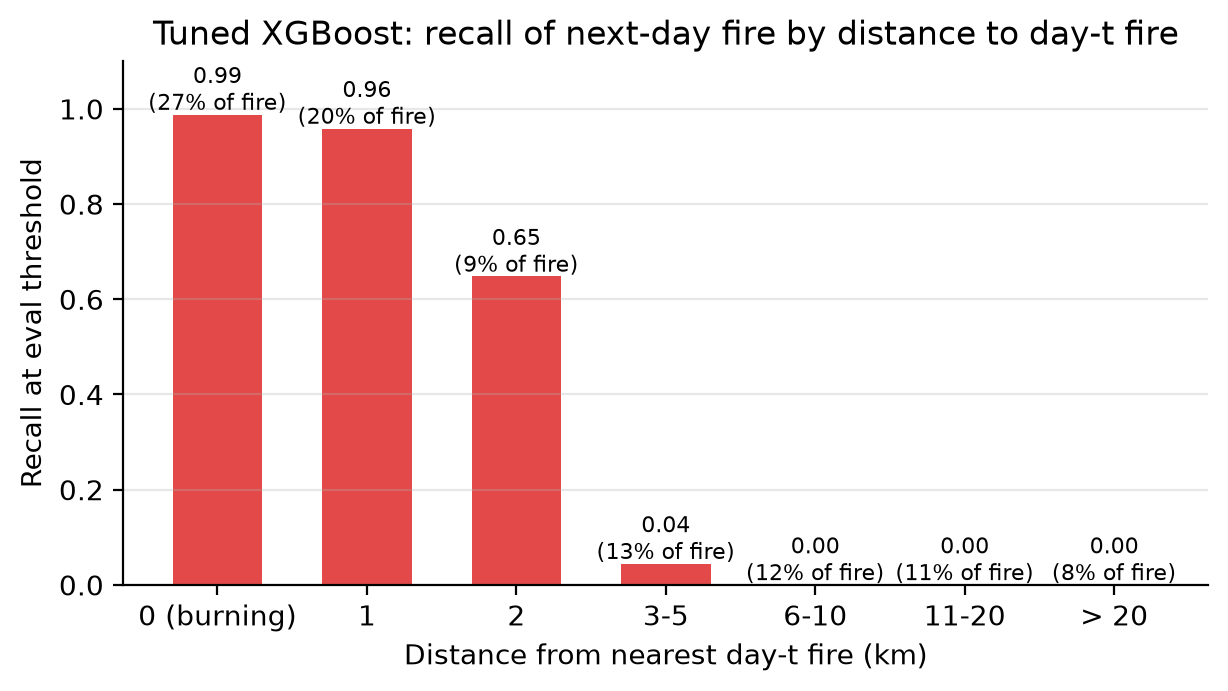
\includegraphics[width=\columnwidth]{figures/eval_recall_by_distance.png}
\caption{Recall of next-day fire pixels by distance to the nearest day-$t$ fire (tuned XGBoost, eval threshold).
Labels give the share of all next-day fire in each band.}
\label{fig:dist}
\end{figure}

At the eval threshold the tuned XGBoost makes 44\,409 true positives, 138\,714 false positives and 39\,922 false
negatives. \textbf{False positives} form a halo around dying fires: 88.8\% lie within 2\,km of day-$t$ fire, and 53.1\%
come from patches whose fire shrinks, although only 38.4\% of test patches shrink; only 35.3\% of day-$t$ fire pixels still
burn on day $t+1$. The five worst patches all hold large, scattered fires (255--468 burning pixels) that shrink the next
day. Nothing in the inputs says which fires will die down (no burnt-out fuel, containment or next-day weather).
\textbf{False negatives} come from long-range spread and sudden growth. Recall falls sharply with distance from the
day-$t$ fire (Fig.~\ref{fig:dist}): 0.988 for burning pixels, 0.959 at 1\,km, 0.648 at 2\,km, 0.044 at 3--5\,km and zero
beyond 5\,km, where 64.4\% of all missed pixels lie. In one patch a fire grows from 8 to 260 pixels in a day and the
halo covers only its centre.

\subsection{Event-level evaluation}
\label{sec:events}

The test split contains duplicate patches and overlapping crops of the same fire, so pooled pixels over-weight large
fires. As the dataset has no fire identifier, we link two test patches when a $16\times16$ elevation block of one
appears exactly inside the other, and treat linked patches as one event. The 1\,689 patches form only 257 events; the 10
largest hold 57\% of next-day fire pixels. Scored per event (240 events with both classes), the tuned XGBoost reaches a
mean PR AUC of 0.187 and a median of 0.120, and the baselines 0.074--0.101, so the ranking holds. At the eval threshold,
however, it finds fire in only 47.9\% of events against 60.8\% for persistence: a threshold that maximises pooled F1 is
driven by the large fires.

\subsection{Limitations and motivation for Phase~2}
A per-pixel model with neighbourhood summaries learns a halo of roughly fixed radius around the day-$t$ fire. It has no
notion of the shape of the fire front, it cannot predict spread beyond a few kilometres, and it cannot tell a growing
fire from a dying one; these are exactly its errors. The hand-made wind features carry real but small signal.
Phase~2 therefore moves to a CNN / U-Net that sees the whole patch, including the fire front and the wind field,
as spatial input.

% Conclusion and Future Work
% Numbers come from reports/results_table.md, reports/ablation.csv, reports/checks and the Results section.

\section{Conclusion and Future Work}
\label{sec:conclusion}

\subsection{Summary}
We predicted next-day wildfire spread on the NDWS dataset with per-pixel gradient-boosted trees and
engineered spatial features. The tuned XGBoost reaches a test PR AUC of 0.257 and a ROC AUC of 0.906,
against 0.145-0.157 for models trained on the raw channels and 0.106 for persistence. At a 5\% false
positive rate it finds 68\% of next-day fire. LightGBM scores 0.248, so the result depends on the
features more than on the boosting library. Our score lies between the neighbour-feature random forest
of Huot et al.\ (0.225) and their CNN (0.284), and below recent U-Nets on the same split (0.346 in a
preprint~\cite{esparza2026}). Since these models come from different pipelines, this places our result
rather than ranking it, and our 95\% bootstrap interval over fire events (0.188-0.325) contains both of
Huot et al.'s values.

Three findings explain this result. First, the spatial features carry the signal. With fixed
hyperparameters, removing the fire-neighbourhood group drops PR AUC from 0.248 to 0.048, and that group
alone already reaches 0.218. Twenty random configurations per model changed eval PR AUC by only about
0.01, and training on 20 times less data gives almost the same eval score, so the remaining error lies
in the input representation rather than in tuning or data size. Second, the model behaves
physically: risk falls with distance to fire, rises with dry air and strong wind, and is pushed
downwind. In the training data, next-day fire 5\,km downwind is up to 3.1 times more frequent than
5\,km upwind in strong wind (Results section). Third, correct evaluation matters at 1\% prevalence. PR AUC, thresholds chosen on eval,
and scores per fire event give a much more honest picture than accuracy or ROC AUC.

\subsection{Limitations}
A per-pixel model with fixed-radius summaries learns a halo around today's fire. Recall is 0.99 for
pixels already burning, 0.65 at 2\,km and zero beyond 5\,km, where 64\% of the missed fire lies. False
alarms gather around fires that die down the next day: 89\% lie within 2\,km of day-$t$ fire, and
nothing in the inputs says which fires will be contained. Scored by event, the model still beats every
baseline (mean PR AUC 0.187), but at the pooled F1 threshold it finds fire in only 48\% of events,
fewer than persistence (61\%). Its raw scores are shifted by subsampling and class weighting. Undoing the shift in closed form gives
probabilities close to the observed fire rate overall, but up to about 3 times too low for the lowest-risk
pixels.

Two limits concern the evaluation itself. Every model was trained once, with one seed, on one split.
Resampling fire events gives wide intervals (0.188-0.325 for XGBoost) because a few large fires hold most
of the fire pixels. Paired resamples still separate the models (Appendix~\ref{app:checks}), and a rebuild
on another machine reproduced every PR AUC within 0.002. The week-based split separates samples in time, but a long-lived fire can appear in
weeks assigned to different splits, and we have not checked how often this happens.

\subsection{Future work: Phase~2}
Phase~2 moves the spatial reasoning from hand-made features into the model. A convolutional
network such as U-Net~\cite{ronneberger2015} sees the whole patch, including the shape of the fire
front and the wind field, which is exactly what the per-pixel model lacks. Because such a network
computes its loss on every pixel, it must handle the full 90:1 imbalance, and focal
loss~\cite{lin2017} is a natural candidate. Further directions are multi-day inputs (the best model on
WildfireSpreadTS uses five input days~\cite{gerard2023}); decision thresholds chosen per event, so that
small fires are not ignored; and calibration checked per region and fire size, so that the
probabilities can be read as risk.

% Appendix: derivations for the Theoretical Background (Priyanshu)

\appendices

\section{Derivations for Section~\ref{sec:theory}}
\label{app:derivations}

This appendix derives the results used in Section~\ref{sec:theory}. Table~\ref{tab:notation} lists the
notation.

\begin{table}[h]
\centering
\caption{Notation.}
\label{tab:notation}
\small
\renewcommand{\arraystretch}{1.12}
\begin{tabular}{l>{\raggedright\arraybackslash}p{5.6cm}}
\toprule
\rowcolor{tblhead}
\textbf{Symbol} & \textbf{Meaning} \\
\midrule
$\mathbf{x}_i,\ y_i$ & features and label (1 fire, 0 no fire) of pixel $i$ \\
$F,\ f_m$ & ensemble score (log-odds); the $m$-th tree \\
$p = \sigma(F)$ & predicted fire probability \\
$T,\ w_j$ & number of leaves; value of leaf $j$ \\
$\lambda,\ \gamma$ & L2 penalty on leaf values; penalty per leaf \\
$g_i,\ h_i$ & gradient and Hessian of the loss for pixel $i$ \\
$G_j,\ H_j$ & sums of $g_i$ and $h_i$ over the rows in leaf $j$ \\
$\pi$ & true fire rate (prevalence) \\
$r,\ w$ & share of no-fire rows kept; weight on fire rows \\
$P,\ N$ & number of fire and no-fire pixels \\
\bottomrule
\end{tabular}
\end{table}

\subsection{Gradient and Hessian of the log loss}
\label{app:grad}

For one pixel, $l = -[\,y \log p + (1-y)\log(1-p)\,]$ with $p = \sigma(\hat{y})$. The sigmoid satisfies
$\partial p/\partial \hat{y} = p(1-p)$, so by the chain rule
\begin{align}
g &= \frac{\partial l}{\partial \hat{y}}
  = -\left[\frac{y}{p} - \frac{1-y}{1-p}\right] p(1-p) \nonumber\\
  &= -\big[\,y(1-p) - (1-y)p\,\big] = p - y , \\
h &= \frac{\partial g}{\partial \hat{y}} = \frac{\partial p}{\partial \hat{y}} = p(1-p) .
\end{align}
So $g$ is the prediction error, and $h$ is largest when the model is unsure ($p = 0.5$) and goes to zero
when it is confident. With weight $w$ on the positive class, a positive row has loss $-w \log p$, and the
same steps give $g = w(p-1)$ and $h = w\,p(1-p)$: both are multiplied by $w$, as in
(\ref{eq:weighted_gh}).

\subsection{Leaf values and split gain}
\label{app:gain}

Substituting the second-order expansion into (\ref{eq:objective}) and dropping terms that do not depend
on $f_m$,
\begin{multline}
\mathcal{L}^{(m)} \approx \sum_{i=1}^{n} \Big[ g_i f_m(\mathbf{x}_i) + \tfrac{1}{2} h_i f_m(\mathbf{x}_i)^2 \Big] \\
+ \gamma T + \tfrac{1}{2}\lambda \sum_{j=1}^{T} w_j^2 .
\end{multline}
Every row in leaf $j$ has $f_m(\mathbf{x}_i) = w_j$, so the sum over rows becomes a sum over leaves,
which gives (\ref{eq:leafsum}). Each leaf's term is a quadratic in $w_j$ with minimum at
$w_j^\ast = -G_j/(H_j+\lambda)$. Substituting it back,
\begin{align}
G_j w_j^\ast + \tfrac{1}{2}(H_j+\lambda)\, (w_j^\ast)^2
&= -\frac{G_j^2}{H_j+\lambda} + \frac{1}{2}\frac{G_j^2}{H_j+\lambda} \nonumber\\
&= -\frac{1}{2}\frac{G_j^2}{H_j+\lambda} ,
\end{align}
which gives $\mathcal{L}^\ast$ in (\ref{eq:leafweight}). A split replaces the parent's term by the terms
of its two children and adds one leaf (one more $\gamma$). The decrease in $\mathcal{L}^\ast$ is therefore
the gain (\ref{eq:gain}).

\subsection{Probability shift from subsampling and weighting}
\label{app:shift}

Let $f_1(\mathbf{x})$ and $f_0(\mathbf{x})$ be the feature distributions of fire and no-fire pixels. By
Bayes' rule the true probability of fire is
\begin{equation}
p = \frac{\pi f_1(\mathbf{x})}{\pi f_1(\mathbf{x}) + (1-\pi) f_0(\mathbf{x})} .
\end{equation}
Keeping a share $r$ of the negatives and weighting positives by $w$ changes the class prior seen by the
loss to $w\pi : r(1-\pi)$, but leaves $f_1$ and $f_0$ unchanged. The probability that minimises the
training loss is therefore
\begin{equation}
p' = \frac{w\pi f_1(\mathbf{x})}{w\pi f_1(\mathbf{x}) + r(1-\pi) f_0(\mathbf{x})} .
\end{equation}
Taking odds, the densities appear in the same ratio in both:
\begin{align}
\frac{p'}{1-p'} &= \frac{w\pi f_1(\mathbf{x})}{r(1-\pi) f_0(\mathbf{x})}
= \frac{w}{r}\cdot\frac{\pi f_1(\mathbf{x})}{(1-\pi) f_0(\mathbf{x})} \nonumber\\
&= \frac{w}{r}\cdot\frac{p}{1-p} .
\end{align}
On the log-odds scale this is a constant shift, $\operatorname{logit} p' = \operatorname{logit} p + \log(w/r)$.
Solving for $p$ gives the inverse map (\ref{eq:inverse_shift}). For our values, $w/r = 89.9$, so a score
of $p' = 0.915$ (odds 10.8) has true odds $10.8/89.9 = 0.12$, that is $p = 0.107$.

\subsection{Precision as a function of prevalence}
\label{app:prec}

Substitute $\mathrm{TP} = \mathrm{TPR}\cdot P$ and $\mathrm{FP} = \mathrm{FPR}\cdot N$ into the precision,
then divide numerator and denominator by $P+N$:
\begin{align}
\mathrm{Precision} &= \frac{\mathrm{TPR}\cdot P}{\mathrm{TPR}\cdot P + \mathrm{FPR}\cdot N} \nonumber\\
&= \frac{\pi\,\mathrm{TPR}}{\pi\,\mathrm{TPR} + (1-\pi)\,\mathrm{FPR}} .
\end{align}

\subsection{Variance of an average of trees}
\label{app:var}

For $B$ trees with variance $\sigma^2$ and pairwise correlation $\rho$, the variance of the sum is the sum
of the $B$ variances and the $B(B-1)$ covariances $\rho\sigma^2$:
\begin{align}
\mathrm{Var}\Big(\frac{1}{B}\sum_{b=1}^{B} \hat{f}_b\Big)
&= \frac{1}{B^2}\Big[ B\sigma^2 + B(B-1)\,\rho\sigma^2 \Big] \nonumber\\
&= \frac{\sigma^2}{B} + \frac{B-1}{B}\,\rho\sigma^2
 = \rho\,\sigma^2 + \frac{1-\rho}{B}\,\sigma^2 .
\end{align}


\bibliographystyle{IEEEtran}
\bibliography{references}

\end{document}
